\documentclass[10pt,titlepage,a5paper]{book}

% \usepackage[babel,german=quotes]{csquotes}
 
 \usepackage[ngerman]{babel}
  \usepackage[utf8]{inputenc}
  \usepackage[T1]{fontenc}


 \usepackage{graphicx}
 \usepackage{geometry}
 \usepackage{pstricks}
 
% \usepackage[style=numeric-comp,backend=bibtex]{biblatex}
% \addbibresource{Bilbliothek.bib}
 
 \pagestyle{plain}
 
%\frenchspacing 

\parindent0em 
\parskip1.0ex plus 0.5ex minus 0.5ex
\sloppy

\geometry{left=2.5cm,right=2cm,bottom=3.5cm,top=2.0cm}

 \author{von\\[0.8ex]Felicitas Stotz}
 \title{\bf\Huge Die Horussöhne}
 
 \newcommand{\sterne}{\par{\centering ***\par}}

 \newenvironment{tg}{\begin{quote}\em}{\end{quote}}
  
 \newenvironment{dichter}{\begin{flushright}}{\end{flushright}}

\newcommand{\changefont}[3]{
\fontfamily{#1} \fontseries{#2} \fontshape{#3} \selectfont}



 \begin{document}
% .
% \newpage
% \newpage
 
 \changefont{ppl}{m}{n}
 
  %\maketitle
   
 \begin{titlepage} 

%\includegraphics[width=0.9\textwidth]{/home/felicitas/133_1.JPG}

\begin{pspicture}
(-4.9,8.5)
\rput(0cm,0cm){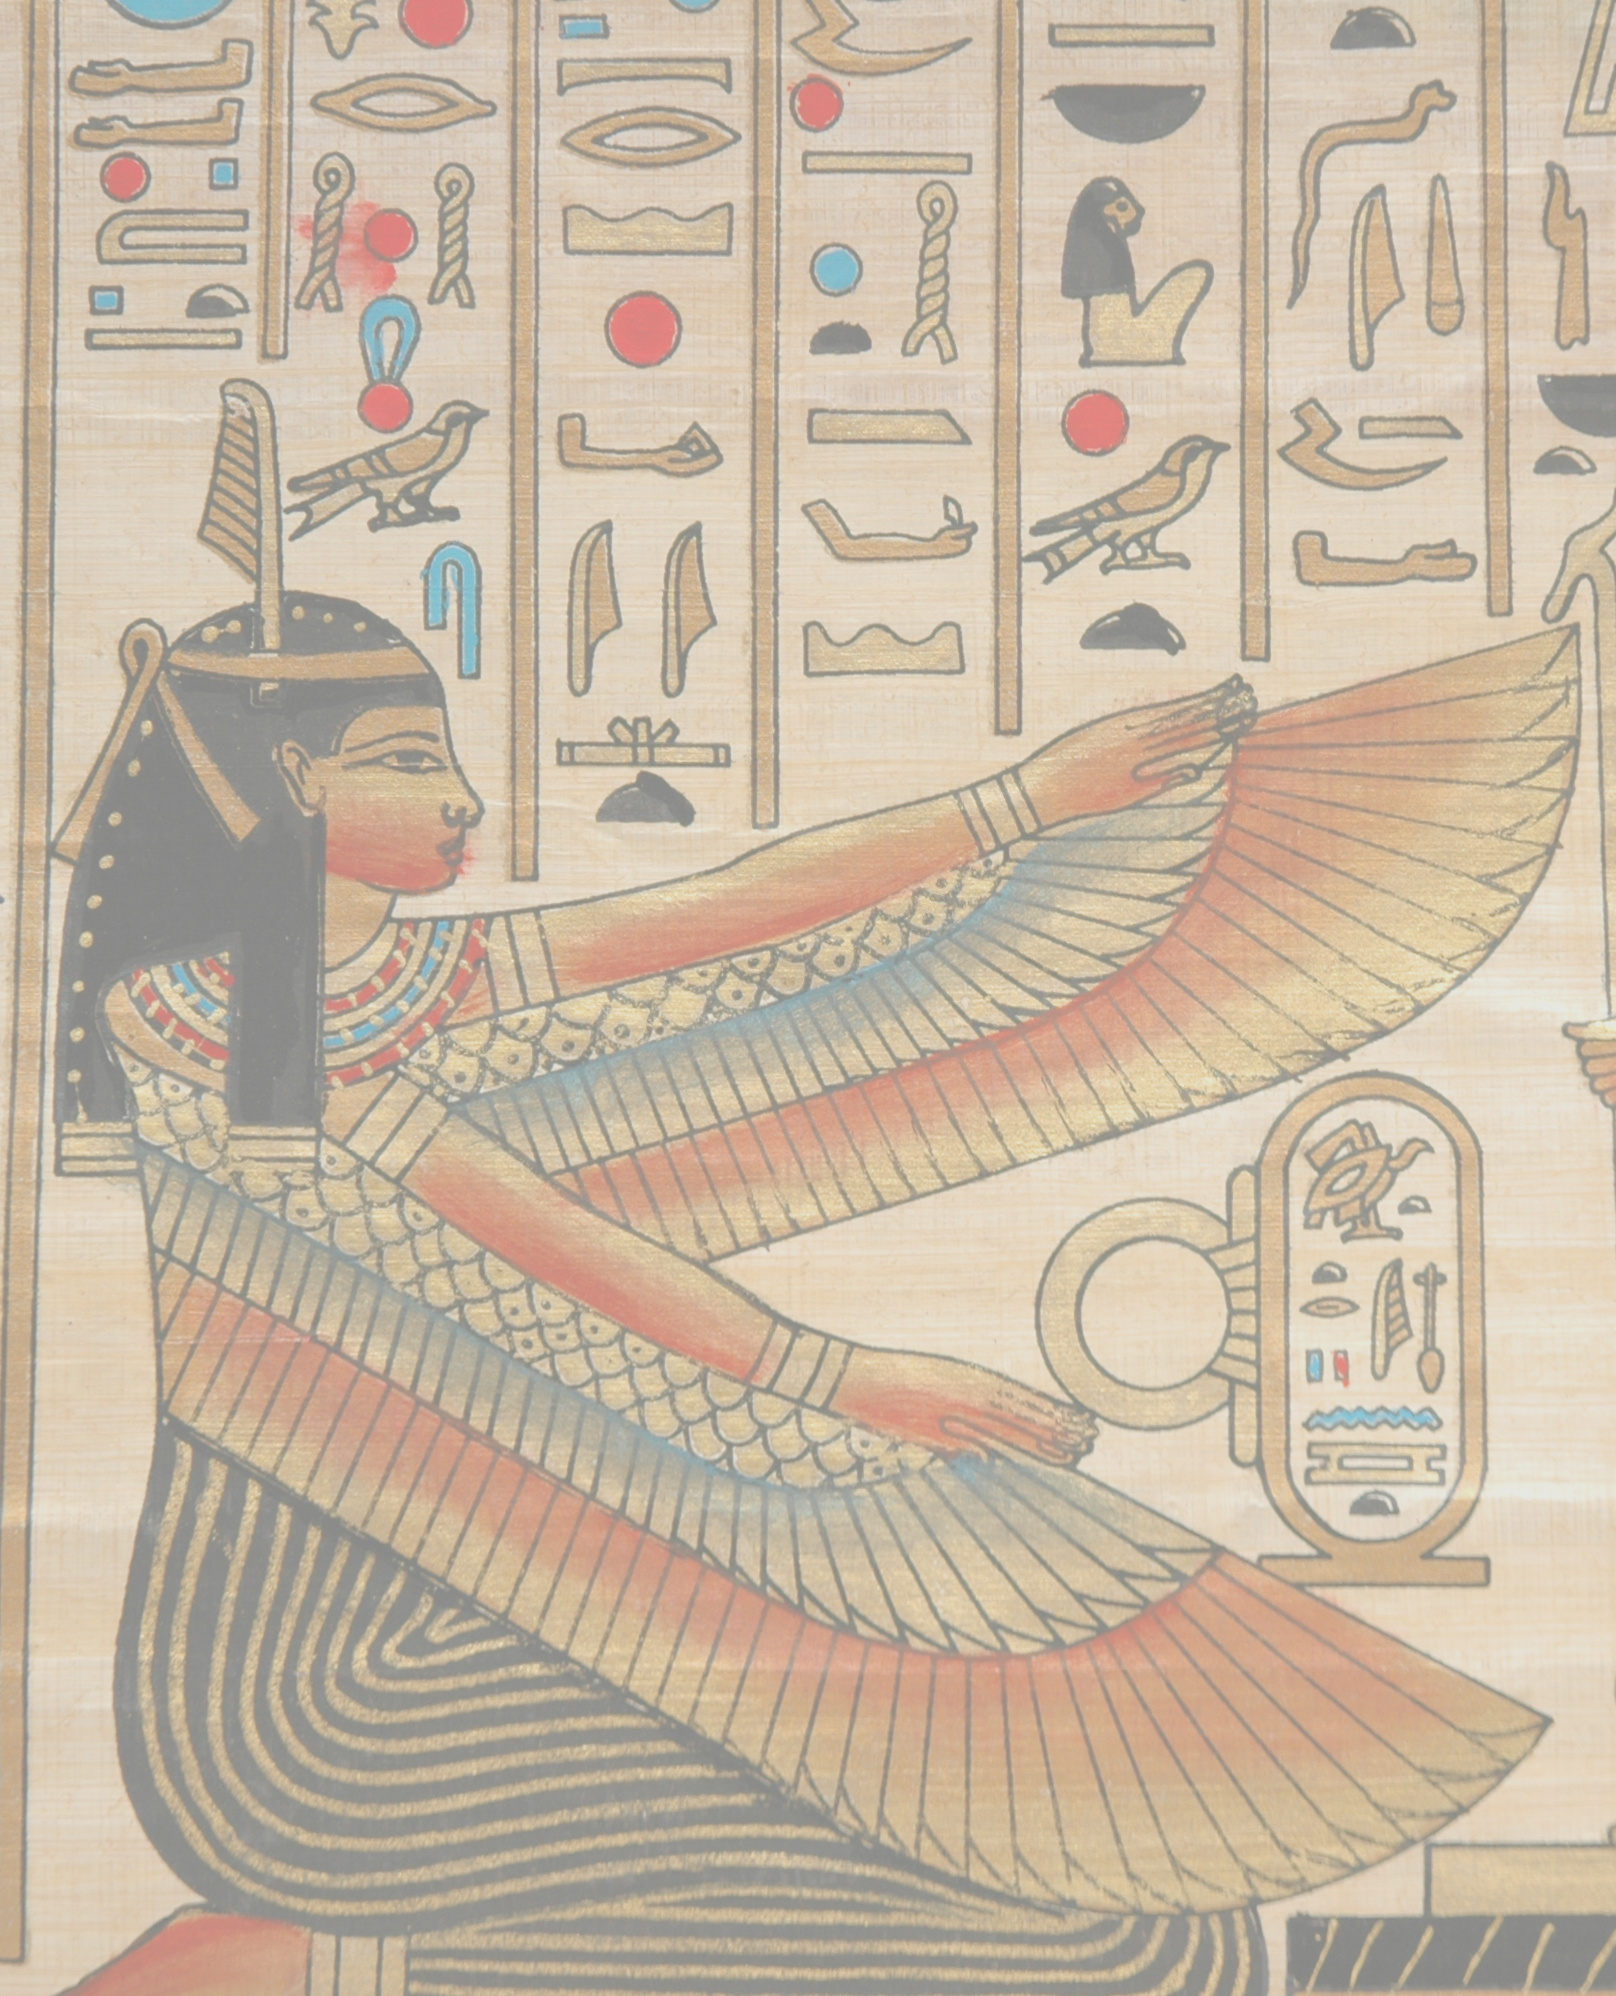
\includegraphics[width=\paperwidth,height=\paperheight]{Titel-Hell}}
\end{pspicture}
 
  \vspace*{-0.5\textheight}
   {\Huge\bf Die Horussöhne}\\[1.5ex]
   Felicitas Stotz\\[24.0ex]
   \today
 
 \end{titlepage}


\thispagestyle{empty}


\chapter*{}

\section*{Titelei}

\begin{tg}
\begin{verse}



Die Schrift des Verborgenen Raumes.\\
Die Standorte der Bau und der Götter,\\
die Schatten und Achu, und was getan wird.

Der Anfang ist das Horn des Westens,\\
das Tor des Westhorizontes;\\
das Ende ist die Urfinsternis,\\
das Tor des Westhorizontes.

Zu kennen die Unterweltlichen Bau,\\
zu kennen die Geheimen Bau,\\
zu kennen die Tore\\
und die Wege, auf denen der Grösste Gott wandelt.

Zu kennen, was getan wird,\\
zu kennen, was in den Stunden ist, und ihre Götter,\\
zu kennen den Lauf der Stunden, und ihre Götter.


Zu kennen ihre Verklärungen des RE,\\
zu kennen, was er ihnen zuruft,\\
zu kennen die Gedeihenden und die Ver\-nich\-te\-ten.{}\\

\end{verse}
\end{tg}



\chapter*{Eine Nacht im Januar(Prolog)}
\addcontentsline{toc}{chapter}{Prolog: Eine Nacht im Januar}


Dies ist die Geschichte einer Reisegruppe. Da diese Reisegruppe aus Göttern der alten ägyptischen Pharaonenzeit besteht, die das schöne Basel in der Schweiz des 21. Jahrhunderts besuchen, handelt es sich um eine ungewöhnliche Reise und um ungewöhnliche Ereignisse und Abenteuer. 

Alle Götter lieben es kreativ und innovativ zu sein, deshalb beginnen sie stets mit dem Anfang, der Schöpfung. 

Das All!  Nicht das All, das wir kennen mit all den Lichtern und Blinkesternen, sondern das All vor Urzeiten, jung und neu. Wir sitzen in einem Raumschiff und beobachten, was passiert. Es ist dunkel, wie in Mutters Schoss. Die Panoramascheibe unseres Raumschiffes ist auf Nachsicht eingestellt. Alter Astronautentrick, um die Geburt von Planeten am Anfang allen Daseins und vor der Erschaffung des Lichtes zu beobachten.

Von der Kaffeemaschine tropft ein einzelner Tropfen herab, wir angespannt, zucken zusammen\dots und vor uns taucht majestätisch und langsam ein riesiger Planet auf. Er befindet sich an der Stelle, wo heute unsere Sonne ist und füllt den gesamten Platz zwischen Sonne und Saturn, so gross ist er. 

Langsam dreht er sich und wir bemerken unterschiedlich stark strahlende Felder. Wir sehen ein Zentrum in der Mitte, von einem helleren umgeben und eine abschliessende Hülle darum. Eiförmige Gebilde  bewegen sich in dem Planeten. Wir schauen auf den Zeitmesser, der sich rasend durch die Zeit bewegt und 1000 Jahre in einer Millisekunde vorbeiziehen lässt. Die Zeit wird langsamer und wir schauen wieder raus. Es wird dunkler, es scheint als verlösche der riesige Planet. Nachdem er verschwunden ist, beschleunigt der Zeitmesser erneut. 

Und plötzlich erscheint vor unserem Panoramafenster ein neuer Planet an Stelle des alten. Dieser Planet ist kleiner und gasförmig. Wir können die Wärmesicht abschalten, wir sehen ihn wunderschön durch die Scheibe leuchten, wir tragen Sonnenbrillen, so hell leuchtet der Planet. Er strahlt glühend, leuchtend weiss, bis auf einige rauchig-dunkle Stellen, die aus Gas bestehen und dichter sind als der Rest. An einigen Stellen ballt sich Wärme, wie wir sie auf dem vorherigen Planeten gesehen haben.

Dieser Planet scheint zu atmen. Eine Zeitlang strömt das Licht weit in das All hinein. Angesogen von einer unsichtbaren Kraft und wird feiner und heller. Dann zieht es sich in das Zentrum zurück, dabei wird es dunkler, dichter, wie rauchige Luft. Kleine Gebilde kristallisieren sich darin, noch können wir sie nicht erkennen. Später werden sie die Sterne des Tierkreises bilden.

Wir haben die Zeit vergessen. Ein Blick auf unsere Zeitanzeige verrät uns, es sind Millionen Jahre vergangen. Wir schauen auf den Planeten und dieser ist wiederum in der Dunkelheit verschwunden.

Wir haben kurz Zeit uns einen Kaffee zu kochen und ein Schnittchen zu machen, da taucht an der Stelle ein neuer Planet auf. Er reicht von der Sonne bis zum Mars. Er ist fester als sein Vorgänger und schillert in allen Regenbogenfarben. Durch den Farbschleier sehen wir Nebel und durch den Nebel sehen wir zum ersten mal so etwas wie Leben. Eine grünliche Masse, wie gekochter Spinat, die lebendig ist und ab und zu ein "`Blubb"' von sich gibt\dots

Wir haben nicht viel Zeit dieses farbenprächtige Bild zu geniessen, denn die Masse des Planeten und die ganze Umgebung drumherum geraten in Aufruhr. Unsichtbare Kräfte reissen den Planeten auseinander. Während gleichzeitig das Universum von unsichtbaren Riesenhänden zusammengepresst wird. Zeitschlaufen öffnen sich und verschlucken Materie in dunklen Röhren, um sie an anderer Stelle auszuspucken. Unsichtbare, unglaublich starke Kräfte kämpfen gegeneinander. Trümmer fliegen herum, Feuerstürme toben, Luftlawinen wälzen sich durch den Raum.

Unser kleines Raumschiff ist zu dicht an dem Geschehen dran, es wird gepackt und geschüttelt. Wir purzeln durcheinander, es gibt eine riesige Kaffeesauerei und die lecker Schnittchen kleben an den Wänden. Draussen sehen wir Blitze, Gaswolken. Druckwellen schütteln uns. Ein riesiges Durcheinander findet statt. Der ursprüngliche Planet ist nicht mehr zu sehen.

Würden wir die alten Mysterien kennen, die ganze Ewigkeiten und durch viele Kulturen hindurch weitergegeben wurden, z.B. die Bhagavat Gita, würden wir wissen, in was wir hineingeraten sind: Den berühmten "`Streit im Himmel"'. Berühmt und berüchtigt, weil er die Geburt des Bösen beschreibt, das zu diesem Zeitpunkt nicht böse ist, sondern getrennt und allein.

- Gespenstische Stille-

Wir klopfen uns die Kleider ab, der Lehrling wird geschickt den Wischmop zu holen und die Kaffeepfützen zu entfernen und eine traurige Schinkenschnitte fällt von der Decke herunter.

Draussen hat es sich beruhigt, aber, was für ein Anblick!

An der Stelle des Planeten sehen wir eine Sonne, sie reicht nicht mehr bis zum Mars, dafür befindet sich auf der Marsumlaufbahn ein Mond. Er umkreist die Sonne und. Was auch immer die Turbulenzen verursacht hat, hat einen riesigen Ring an Trümmern hinterlassen, den Asteroidengürtel, den wir später zwischen Mars und Jupiter finden!

Die Sonne leuchtet hell und ist leicht, während sich auf dem Mond die Materie zu Luft und Wasser verdichtet. Auch hier schillern wieder die Regenbögen und der lebendige Spinat macht "`Blubb"'\dots

Ein letzter "Neustart" findet statt, Licht aus, Licht an und vor uns taucht die Erde auf. Sie ist viel grösser, denn es werden sich aus ihr Uranus und Saturn herauslösen, bevor sie sich endgültig verfestigt hat. Als nächster trennt sich der Jupiter und dann der Mars.

Wir können es nun wagen auf das Raumschiff zu verzichten, auch wenn wir bei der jetzigen Erdatmosphäre vermutlich einen Raumanzug nötig hätten, mit unserer heutigen Gestalt.
Ein letzter Blick auf den Zeitmesser, dort ist an Stelle der Zahlen eine Schrift erschienen: Genesis, Tag 1

Die Sonne verlässt die Erde und später, als letztes der Mond. Nachdem es sich die Planeten alle für diese Runde gemütlich gemacht haben, tritt das erste mal gross auf die Bühne in physischer Gestalt: Der Mensch.

Natürlich waren wir Menschen schon vorher da, wir waren auch dabei, als der Wärmeplanet sich im All begann zusammenzuballen, aber wir hatten kein Bewusstsein und nichts womit wir eines hätten haben können. Dieses Bewusstsein brauchte all die vielen Zeitrotationen auf unserem Zeitmesser, Millionen von Jahre und mehrere Äonen von Heimatplaneten, bevor es soweit war.

Und dann kam Atlantis. (Womit unsere Geschichte, der Leser möge den schmählichen, aber einkalkulierten Fauxpas verzeihen, einen Gènréwechsel von Science-Fiction zu Fantasy durchmacht, kommt nicht mehr vor, versprochen.)

Götter sind kreativ und eine ihre beliebtesten Hauptaufgaben ist die Schöpfung. Es gibt viele verschiedene Versionen und Ideen bei den Menschen, wie die Erde in den Zustand gekommen ist, in dem sie sich zur Zeit befindet. Und viele Jahrtausende waren sich die Menschen einig, es sind Götter gewesen. Einer, viele, egal, aber Götter. Unsichtbare, dem Menschen überlegene Wesen, die alles mehr oder weniger leiteten und im Griff hatten.

Heute, nur am Rande bemerkt, lachen die Menschen über dieses Konzept. Sie glauben nicht an Götter, sondern an die Wissenschaft, was bedeutet, alles hat sich entwickelt. Wie genau das gegangen ist, ist so kompliziert, das verstehen nur wenige (früher nannte man die Wenigen mit dem "`geheimen Wissen"' "`Eingeweihte"' und dieses Wissen wurde eifersüchtig von ihnen gehütet, aber das war früher). 

Wenn wir verschiedene Schöpfungsgeschichten anschauen, werden wir feststellen, Götter sind nicht nett. und in diesem Sinne, liegt auch in unserer Zeit die Frage nahe, ob der Mensch nicht doch göttlichen Ursprunges ist.\footnote{Das liegt näher, als die Vermutung, einiger heutiger "`Eingeweihter"', die glauben, der Mensch sei ein Affe. Aber die Affen können nichts für den Zustand der Erde und es ist gemein, sie ungefragt in die Sache mit der Erde und den menschlichen Zerstörungsversuchen mit hinein zu ziehen. Das haben sie nicht verdient, für ihre Ähnlichkeit mit den Menschen können sie schliesslich nichts.}

Unsere Geschichte der göttlichen Reisegruppe beginnt an einer Stelle der Schöpfung, als die Menschheit sich an einem ähnlichen Punkt befand wie wir heute, wenn wir alten Überlieferungen glauben. Natürlich war dennoch alles anders:

Nebelverhangen war das Land Atlantis. Die Menschen besassen weder einen Körper, wie wir ihn kennen, noch hatten sie unser heutiges Bewusstsein. Die Menschen, sie träumten, sie fühlten sich, wenn sie wach waren, wie wir uns heute im Schlaf fühlen. Dabei waren die Atlantier hoch begabt, sie konnten etwas, was uns heute nicht mehr möglich ist. Sie waren hellsichtig und konnten die Kräfte, die im Pflanzen- und Mineralreich vorhanden waren, auf diese Weise nutzten. Auf diese Weise fuhren sie in Fahrzeugen herum, die mit der Kraft von Steinen angetrieben waren. Unvorstellbar? 

Eigentlich nicht. Wir können die Kräfte der Natur, dank unserer weit entwickelten Fähigkeit zu denken, nutzen. Schauen wir ein Auto an, wir nutzen  Pflanzen- und Mineralkraft, indem wir das Auto aus Metall (Mineralien) bauen und mit Erdöl (Pflanzen) in Bewegung setzten.

Was die Atlantier jedoch tatsächlich unterschied und was uns heute am seltsamsten anmutet würde, ist nicht ihr merkwürdiger, zu Beginn dieser Zeit knochenlose Körper und ihre Hellsichtigkeit, die ihnen ein ähnlich komfortables, weitentwickeltes Leben wie uns heute, bescherte. Leute, stellt Euch vor, die hatten ihre Smartphones praktisch integriert;) Nein, der grösste Unterschied war, sie kannten ihre Götter! Persönlich. Mit Vor- und Nachnamen und Adresse! (Was nicht viel half, denn wie wir wissen, ging Atlantis kläglich unter.)

Einer, der nicht unterging, so sagt es die Legende, weil er weise war und sich deshalb dem Wohlwollen der atlantischen Götter erfreute, war Thot. Thot konnte vor dem Untergang der Atlantis flüchten. Und der damals sehr begabte, aber menschliche Thot floh nach Ägypten und fand dort für sich und sein geheimes, atlantisches Wissen eine neue Heimat.

 Thot wurde später selbst Gott im Ägypterland und war auch bei den Griechen kein unbekannter. Im Gegenteil, sie nannten ihn, wiederum nach ihrem Gott Hermes: Hermes Trismegistos. Wer jetzt im hinterletzten Winkel seines Gehirns ein leises Klingeln hört, das sich wie "`hermetisch"' anhört, dem wird dämmern, wie weitreichend Thots Einfluss war und ist. Dabei ist er nicht der mächtigste der ägyptischen Götter\dots


Er ist allerdings der Gott, weil mit dem Menschlichen wohl vertraut, der sich am besten als Reiseleiter eignet. Für eine Reisegruppe von Göttern, die teilweise nicht über menschliche Körper verfügen, oder nie aus dem Jenseits, der ägyptischen Duat herausgekommen sind, ist es von Vorteil einen gut informierten Reiseleiter zu haben.

 Der Jenseitsbereich ist um die Erde herum, ein riesiger Raum für alle Götter, die für die Erde zuständig sind. Allerdings haben die Götter des einen Zeitalters und/oder des einen oder anderen Landes ihre ganz spezifischen Aufgaben und nicht alle wollen sich um alles kümmern. Andere haben sich auf den "`Altenteil"' zurückgezogen und geben den jüngeren Göttern Tipps, wie man tüchtige Blitze schleudern kann, ohne dabei die ganze Gemeinde auszulöschen.
 
 Wenn sich die Menschen jedoch anmassen, sich einem Gott zu widersetzten, oder einen unbestechlichen Wächtergott auf grausame Weise hintergehen und seinen Schutzbefohlenen schaden, dann können auch alte Götter sich für eine Reise entschliessen. Und nicht alle Götter scheuen sich, ihre Kollegen um Hilfe zu bitten. Und so kommt es, dass der grosse Hermes Trismegistos, der "`dreimal grosse Hermes"' genannte Thot, gleich in dreifacher Mission nach Basel kommt. 
 
Thot kennt seine Pappenheimer an jedem Ort. In Basel einen Wohnort für sein buntes Reisegrüppchen zu finden ist einfach. Was liegt näher als die Damen und Herren an dem Ort unterzubringen, an dem ein ehemaliger Adept der Alchemie und Hermetik seinen grossen Auftritt hatte: der grosse Cagliostro? Für die einen ein Scharlatan und für die anderen ein Grossmeister der ägyptischen Logen und Besitzer des Steines der Weisen. Als er am Rheinsprung vor den zwei grossen Häusern der Gebrüder Sarasin steht nickt er zufrieden. Schliesslich wollen auch die abenteuerlustigsten Götter und vorallem Göttinnen nicht auf einen Hauch an Luxus verzichten.

Im berühmten Oktagon, dem achteckigen Zimmer des weissen Hauses des ehrwürdigen Jakob Sarasin, trifft sich der alte ägyptische Gott mit seinen nordischen Freunden Berta, auch bekannt als eine gewisse Frau Holle und Hans, dem "`Wilde Maa"'.

Während Thot sich in einen Ohrensessel gesetzt hatte, von denen zwei im Raum standen, lief Berta im Raum auf und ab. Sie steckte in einem langen schwarzen Kleid und einer weissen Schürze. Sie sah aus wie ein altes, verhutzeltes Hausmädchen. In ihren grauen, kurzen Locken steckt ein weisses Häubchen. Ab und zu schauten ihre Füsse, die in derben, braunen orthopädischen Schuhen stecken unter dem Kleid hervor. Vor der Tür im Gang stand ein Reisigbesen. Ab und zu nahm sie einen Schluck aus dem Kristallglas, das mit einem rauchig duftenden, bernsteinfarbenem Whisky gefüllt war. Es stand auf einem kleinen runden Nussholztischchen.

Ein zartes Grunzen ertönte. Von dem zierlichen mit Seide bezogenem Sofa, schauten nur die geschwundenen, dünnen Beinchen hervor, der Rest war unter  dem wilden Mann begraben. Ausser einem Schurz aus Laub, Fell und Zweigen und einer Krone aus Eichenlaub war er nackt. Seine Haut schimmerte goldbraun und unter der Haut zeichneten sich die kräftigen Muskeln ab. Das Gesicht war faltig und die wilden Locken schimmerten nicht nur braun und grau, sondern grün. Da das Sofa viel zu klein war, hing ein Bein über die Lehne und das andere ragte weit ins Zimmer. Ein Arm hängt auf den Boden und wenn der Wilde Mann schnarchte, zitterten die Blätter seiner Krone hingebungsvoll. 
 
"`Interessant, äusserst interessant!"' Thot legte die schlanken Fingerspitzen aneinander. Er bevorzugte einen zeitgenössischen, schlichten, schwarzen Anzug. Sein Hemd war leicht weiss-grau gestreift und er trug eine hellgraue Krawatte. In einer angesehenen Anwaltskanzlei, wäre er heutigen Tags vermutlich nicht aufgefallen. Er hatte eine schmale, aber lange Nase. Die hellblauen, kristallklaren Augen, lagen tief und waren von der Stirn und den Augenbrauen verborgen. Seine schwarzen Haare lagen wie ein lockiger Helm um seinen Kopf und waren mit grauen Strähnen durchzogen. 

Er hatte die langen, schlanken Beine übereinander geschlagen und wippte unrhythmisch mit dem Fuss. "`Und was schliesst du daraus, verehrte Berta?"' "`Lieber Thot, wenn ich es selber wüsste, hätte ich Euch wohl kaum hierher bemüht!"' sagte Berta und liess ratlos die Arme fallen. Thot sagte entschieden: "`Im Moment werde ich gerne bemüht. Mir ist langweilig geworden im Jenseits und den anderen Herrschaften auch. Wir können Bewegung brauchen, sowohl für den Kopf, als auch für die Beine!"' "`Ich bin sicher, da kann ich dir helfen, Thot. Da ist etwas ganz finsteres im Gange, das hab ich in den Knochen."' 

Berta wendete sich dem mannhaften Laubhaufen auf dem Sofa zu: "`Hans? Hans, was sagst Du dazu?"' "`Wckl? Was?"' es dauerte einige Zeit bis sich der Halbgott sortiert hatte und sich aufsetzte. Er stöhnte, schnaufte und hielt sich den Kopf. Berta betrachtete das Spektakel, die Hände auf die breiten Hüften gestemmt:  "`Herrjeh, dann hat er einmal im Jahr seinen grossen Auftritt und danach ist er Wochenlang nicht zu brauchen! Dir tut etwas mehr Bewegung gut, alter Mann!"' rief sie und fuchtelte Hans mit dem Zeigefinger vor der Nase herum. Er ächzte: "`Alter Mann?! Also nai, Berta, eso nit!"' Er richtete sich zu seiner vollen Grösse auf und sah der kleinen, kugeligen Frau Holle, die feixend vor ihm stand, sitzend direkt in die Augen.

 "`Fein, dann ist es beschlossen?"' Thot schmunzelte, sie waren sich überall ähnlich, die alten Herrschaften \dots Vergnügt nahm er Stück von der feinen Mandelschokolade, die auf einem feinen Porzellanteller für ihn auf dem Tisch bereit stand. 

"`Wo? Ich persönlich würde Basel vorziehen, da ich selbst etwas erledigen will, was in Ägypten nicht möglich ist!"' murmelte Thot mit einem Rest Schokolade im Mund. "`Hans? Was meinst Du?"' Berta, die einen kräftigen Schluck aus ihrem Glas genommen hatte, wendete sich an Hans. "`Basel!"' sagte Hans. 

Er nahm sich das Bierglas, das auf dem Tisch für ihn bereit gestanden hatte: "`Mr mache s in Basel!"' Er schleckte sich mit der Zunge den Schaum von den Lippen und schaute die anderen beiden versonnen an: "`D Basler sind frommi Leut aber heuer hent sie mit sich und ihre Gschäft z tue. Sie sind gnueg igbildt, ihne werde me oder wenigr Göttr do nit uffalle. Und hier z Basel und umgäbig hätts viili Lütt, wo dr Thot kenne und wo ich kenn, und dir, Berta, lieg jo, s Dreiländreck e z Füesse."' Berta warf einen tiefen Blick in ihr Whiskyglas: "`Gut, klingt vernünftig, auch, wenn es von dir kommt!"' "`Berta! Eso, würkli nit!"' meinte Hans freundlich.   

"`Das Wann dürfte allen klar sein?"' fragte Berta. "`Berta!"' rief Hans genervt "`mr sind do keini Deppe!"' "`Natürlich, liebe Berta!"' Thot erhob sich und streckte die langen Glieder. Er war zwar nicht so muskulös wie Hans, aber genauso gross.

"`Ja dann, see you later mit alligator\dots"' Hans lachte grollend. "`Bis Mitwinter!"' rief Berta, die sich den Besen unter den Arm geklemmt hatte und sich Handschuhe überstreifte. "`Es sind Krokodile!"' sagte Thot: "`Keine Alligatoren, sondern Krokodile. Bis Heilig Abend."'

\section*{23. Dezember}
\addcontentsline{toc}{section}{23. Dezember}

"`Hermes, min Fründ, d Berta macht jetzt alles parat für de Transport. Sind dr do z Basel au patrat?"' "`Wir sind bereit, Hans. Unsere grosszügigen Gastgeber, die Brüder Sarasin, haben uns erlaubt im weissen und blauen Haus zu wohnen, die auf das beste geeignet sind."' "`Is' d Alessandro fertig mitmm Schutznetz? Hät er de Zeitüberschneidung richtig usgrechnet?"' "`Ja, ich habe es überprüft. Und unser Alessandro, Graf von Cagliostro, ist ein wahrer Spezialist, wenn es darum geht einen Ort in zwei Zeitzonen einzuteilen. Schliesslich ist diese Fähigkeit sehr nützlich, wenn man, wie er, gerne dem schönen Geschlecht huldigt."' "`Ei, das hesch schön gesagt, dem 'schönen Geschlecht' huldigen\dots so isses, Hermes, d Herr Graf isch kein Kind vo Traurigkeit, ds isch woor!"' 

"`Die Häuser werden in der Gegenwart am Tag benutzt. In den Häusern befinden sich ein Departement der Stadtregierung. Allerdings werden in den Tagen der Rauhnächte weniger Menschen dort sein. Sie stören uns nicht und sehen können sie uns auch nicht. Vielleicht wird der eine oder andere Mensch Kopfschmerzen haben und wirre Träume, aber mit dem können wir leben."' "`Gut"' sagte Hans  "`dann werd` ich Berta sage, dass mr unsern Transport starte könne und ihr helfe, de Route frei z halte und däne Ameise Bein mache. Sind halt scho tolli Tierli. Hermes, mi Fründ, viel Glück bei eurer Reis`, diini Herrschafte sind jo nümmi de jüngschte!"' Hans holte freundlich aus und gab Thot einen Klaps auf die Schulter. Dieser zuckte unmerklich zusammen, es knackte in seinem Bein. "`Du solltest sie sehen"', Thot rieb sich über das Knie, "`die gute Hathor, ist schon seit Wochen am Packen. Sie freuen sich alle auf das Abenteuer."' "`See you\dots"' Hans hob grüssend die Hand. Thot humpelte, möglichst unauffällig, zur Tür. Dort wendete er sich um und sagte lächelnd: "`Es sind Krokodile, Hans. Bis bald."'


\part*{Erste Stunde:\\"`Welche die Stirnen der Feinde des Re zerschmettert"'}
\addcontentsline{toc}{part}{Erste Stunde}


\chapter*{24.Dezember, Adam- und Evatag}
\addcontentsline{toc}{chapter}{24.Dezember; Adam und Evatag}

\section*{1}

Amélie öffnete die Augen, was für ein Traum\dots

Aber, he, das war nicht ihr Zimmer! Wo in aller Welt war sie? Sie zog die weisse Bettdecke, die mit den Daunen von einer Million Gänsen gefüllt war, herauf zur Nasenspitze und rutsche tiefer in das weisse, flaumige Kissen. Sie lauschte, während die Augen das Zimmer durchstreiften. 

Die Wände waren weiss. Eine Kommode aus Nussbaum stand an der einen Wand, daneben war ein Tür, die in ein anderes Zimmer führen musste. Das Bett stand gegnüber. Am Kopfende des Bettes fiel durch zwei grosse Sprossenfenster trübes, graues Winterlicht, in den quadratischen Raum. Durch eine zweite Tür, gegenüber den Fenstern, hörte sie eilige Schritte hin und her gehen. Auf der anderen Seite dieser Tür musste sich ein langer Gang befinden. Das Zimmer schien in einem grösseren Gebäude zu sein. Stimmen waren zu hören aus verschiedenen Richtungen, die einen wie leises murmeln, die anderen laut und dicht.

Das Zimmer roch nach Wachs mit dem der dunkle, alte Holzboden gepflegt worden war. Es roch nicht nur alt, sondern unpersönlich, wie ein Büro- oder Amtsgebäude. Die Geräusche und Stimmen schienen einer aufgeregten Grossfamilie zu gehören.

Amélie streckte sich. Und starrte an die Decke. An der Decke war ein schwarzer Punkt. Ein schwarzer Punkt, der sich bewegte! Eine Spinne? Amélie konnte ein Quietschen nicht unterdrücken und steckte den Kopf unter die Decke. Vorsichtig spähte sie hervor, das Tier war verschwunden! Abgestürzt? Wohin? Auf ihre Decke? Mit einem Schrei, sprang Amélie aus dem Bett. Schüttelte sich wild und hopste durch Zimmer. Wo war die verdammte Spinne?

 Da, da war sie! Über der Kommode! Amélie schnappte ihr dickes Kissen und hob es über den Kopf, bereit auf alles einzuschlagen, was mit einem Bein zuckte. Dann sah sie genauer hin, es war keine Spinne, es war eine Ameise. Überrascht lies Amélie das Kissen sinken und betrachtete das Tier. Eine Ameise? Im Winter? Amélie beugt sich vor, ihre langen, glatten schwarzen Haare rutschen über die Schultern nach vorne. Diese Ameise sah erschöpft aus!

Amélie setzte sich auf das Bett. Erst jetzt bemerkte sie, was für Kleider sie trug, sie hatte ein weisses Unterhemd mit breiten Spitzenträgern und eine weisse Unterhose an. Woher? 

Kalt war es, sie schlang die Arme um sich und zog die Beine an. Sie versuchte sich zu erinnern: War es ein Traum gewesen? Ein Traum mit Ameisen. Sie hatte geträumt, eine riesige Zahl Ameisen würde sie durch einen unterirdischen Gang schleppen. Die Ameisen wurden von einem grossen, kräftigen Mann mit einem dunkelbraunen, struppigen Vollbart und wildem Haar angetrieben, der mit grünem und braunem Laub bedeckt war und von \dots Berta?

 Amélie war betäubt gewesen. Sie konnte sich während des Transportes nicht bewegen und dämmerte auf dem Marsch dahin, der, wie ihr schien, Tage dauerte. Einzig geweckt wurde sie, wenn ihr Kopf oder ein anderer Körperteil unsanft gegen eine Baumwurzel schlug, die  in den erdigen Gang hineinragten. 
 
 Sie erinnerte sich an grässlichen Lärm quietschender Räder auf Schienen. Tunnel, dunkel, betoniert und mit Leitungen vollgestopft. Ein blendendes Licht, S-Bahnen, die direkt auf sie zu gebraust kamen und mitten durch sie, die Ameisen und den fluchenden, wilden Mann durchfuhren, ohne abzubremsen. Sie verschwanden im Tunnelgewirr, Berta schrie und trieb die Ameisen an, während diese Amélie mit dem Kopf gegen die Wand stiessen, bis die Wand nachgab, sich öffnete und sie sich wieder in einem Erdgang befanden.

Es klopfte an der Zimmertür.
"`Hallo? Amélie! Bist Du wach?"' Amélie schlüpfte unter die Decke. Panik machte sich breit, das war eindeutig die Stimme von einem Kerl. Einem jungen Kerl! Sie hörte angespannte Stille, dann schnaufte es vor der Tür. "`Ja! Nein! Stopp!"' rief Amèlie. Aber da stand der junge Mann in der Tür und an ihm vorbei drängelte sich ein graziler, schlanker Hund mit dickem, goldbraunem Fell. Er trug einen schwarz-grauen Sattel aus längerem Haar auf dem Rücken und die Ohren waren spitz und gross. Der Hund war es, der aufgeregt schnüffelte. Er blieb in einiger Entfernung stehen und starrte Amèlie unhündisch an.

"`Ich hab keine Kleider,"' Amélie spürte, wie ihr die Röte ins Gesicht stieg und tauchte tiefer unter das Federbett. "`Ah, oh! Ich glaube Isis hat dir etwas zum anziehen in die Kommode gelegt,"' erklärte der junge Mann eifrig der Bettdecke. "`Ich bin übrigens Amset und das ist mein Bruder Duamutef."' Er strahlte und zeigte auf den Hund\dots

Isis? Bruder? Ein Hund? Bin ich von Verrückten entführt worden? Amèlie reckte ihre Nase vor und rief empört: "`Verschwinde! ich will mich anziehen!"' Amélie nahm das Kissen und warf es. Es prallte an der hastig geschlossenen Tür ab und plumpste zu Boden.

-Haha, sie hat nach fünf Minuten schon den ersten Gegenstand nach dir geworfen, Amset! -Ach, halt dein Maul, Tef! -Hast du gewusst, dass sie dich für verrückt hält? "`Maul halten, Tef!"' Amset war es lauter rausgerutscht, als er wollte -Was schreist Du denn so? Der Schakal kräuselte die Schnauze -Haha! -Und dich hält sie für einen Hund, konterte Amset. Duamutef zog unwirsch die Lefzen hoch.

Der Schakal und der junge Mann stiegen die grosszügige Treppe hinunter. Sie waren Götter und Brüder, der eine war ein Mann und der andere ein Schakal. Wie sie miteinander sprachen? Mit Gedanken! Sie waren vier Brüder, die berühmten Horussöhne, unbestechliche Wächter im Totenreich. Der dritte Bruder Kebechsenuef war ein Falke und der vierte, Hapi, ein Pavian. Und sie waren jung. Und sie hatten Glück, denn Götter sind ewig -z. B. jung.

-Geh raus in den Garten deine Geschäfte machen, Tef! Und Grüss Hapi und Kebi von mir. -Heb' mir was vom Frühstück auf, ja? Der Schakal verschwand durch die Tür, die Amset ihm öffnete, in den Garten.

Amélie tappte auf Zehenspitzen zur Kommode. Aus dem Augenwinkel bemerkte sie eine Bewegung am Fenster. Es war nichts zu sehen. Ausser dem grauen Himmel.

 "`Gib sie her!"' "`Hol sie dir doch! Komm doch! Kooomm!"' "`Isfet, gib sie her, ich bring dich um!"'"`Vergiss es, Maat, das darfst du nicht!"' Die andere Tür flog auf und zwei Mädchen fielen ins Zimmer. Sie wälzten sich am Boden. Die eine von ihnen hielt eine weisse Straussenfeder von sich gestreckt, nach der die andere hektisch griff. Sie bekam sie nicht zu fassen, weil ihre Gegnerin energisch zappelte. Amélie schnappte sich behutsam die Feder und zog sich ans Fenster zurück. "`Gib mir die Feder!"'

Die schlanke Gestalt, etwas kleiner als Amélie, streckte gebieterisch die Hand aus. Sie trug ein gerade geschnittenes, schwarzes Kleid mit weissem Spitzenkragen. Sie hatte weisse Söckchen ebenfalls mit Spitze an, im Winter! Und schwarze Spangenschuhe aus Lack. Die schwarzen Haaren trug sie zum Pagenkopf geschnitten, mit einer weissen Schleife gebunden. Die Haare waren zerzaust und die Schleife hing schief, ihre Wangen waren gerötet. Aber als sie der zarten Gestalt ins Gesicht sah, bekam Amélie eine Gänsehaut.

 Ihre Augen waren gelb. Goldgelb. Und sie strahlten eine machtvolle Würde und Weisheit aus. Amélie schluckte und gab dem Mädchen die Feder, stumm und erschrocken. "`Danke!"' sagte die kleine Person und ging erhobenen Hauptes aus dem Zimmer. 
 
 "`Isfet!"' sagte die andere und streckte Amélie die Hand entgegen. Diese hätte ein Zwilling sein können, allerdings einer, der aus dem Nest der Ordnung gefallen schien. Isfet hatte kurze, verwuschelte, schwarze Haare. Sie steckte in einem riesigen, bunten Sweatshirt mit Kapuze und einem Pinguin drauf, ihre Beine in pinken Leggings mit blauen Tupfen und die Füsse in dicken Stiefeln.
 
"`Amélie,"' sagte Amélie. "`Ich weiss!"' Isfet liess sich auf das Bett fallen. "`Alle scheinen das zu wissen"', maulte Amélie "`und ich weiss nicht mal, wo ich bin. Verdammt, wo bin ich? Und wer seit ihr? Ein Haufen Verrückte?"' Isfet grinste: "`Du bist schon in Ordnung, weisst du das? Zieh dich an und komm runter, dann lernst du den restlichen Haufen kennen."'

Amélie zog die Kommodenschublade auf, da! Da war wieder eine Bewegung am Fenster, sie zuckte zusammen. Isfet jedoch sprang ans Fenster, riss es auf und schrie: "`Kebi, lass' das, sie ist ein Mädchen und ein Gast, n' bisschen Anstand, jaah!"' Sie schloss das Fenster wieder und drehte sich zu der bleichen Amélie. "`Diese Brüder. Wenn sie nicht arbeiten, sind sie immer zu Spässen aufgelegt, die Jungs!"' Isfet ging aus dem Raum und Amélie trat ans Fenster. Auf dem gegenüberliegenden Dach sass ein Raubvogel, ein Falke. Komisch, dachte Amélie, mitten in der Stadt\dots

 Brüder? Hatte jemand von der gegenüberliegenden Seite aus dem Fenster geschaut? Amélie betrachtete das Haus. Es erstreckte sich auf drei Seiten. Zwei Stockwerke war es hoch und im Dach waren viele kleine Gauben mit weiteren, kleinen Fenstern. Blau, weiss war das Haus. Im Innenhof war ein üppiger Garten angelegt mit einem grossen Teich. Seltsamerweise war der Garten grün, die Bäume trugen Laub. Die Bäume verdeckten den offenen Teil, so dass Amélie nicht sah, ob der Garten eingezäunt war und wie die Strasse aussah. Jedenfalls war sie in einer grösseren Stadt, denn es waren weitere Dächer zu sehen und Strassenlärm tönte herauf. Zwischendurch war ein Kreischen zu hören, wie Amélie es aus dem Affenhaus im Zoo kannte.
 
 Energisch zog Amélie die Vorhänge zu und machte sich über die Kleider in der Kommode her. Sie passten ihr wie angegossen und trafen genau ihren Geschmack, jedenfalls etwas, dachte sie und machte sich auf zum Frühstück, wo immer es auch sein mochte. Ach, ja, dachte sie, heute ist Heiligabend!


\section*{2}
\addcontentsline{toc}{section}{2}


Amélie sass im Garten auf einer Marmorbank. Wenn das eine 'harmlose Gruppe von Touristen aus Ägypten' ist, dann bin ich Kaiserin von China, dachte sie. Auch wenn alle betont entspannt und lässig taten. Der eine ältere Typ hatte sogar am Frühstückstisch seine Sonnenbrille anbehalten! Und diese Hathor wollte Amélie Würmer aus der Nase ziehen, dabei wusste sie selbst nicht, wie sie hierher gekommen war. Basel, hatten sie gesagt. Was soll ich bitte in Basel? Und dann war da dieser Typ im schwarzen Anzug, der sprach, als wenn er einen Einstein verschluckt hätte. Der wirkte am normalsten, wenn er nicht so ernsthaft mit seinem grossen, schwarzen Hund reden würde, als ob der alles verstünde, was er sagte. Anubis, hiess der Hund, den Namen hatte Amélie schon in einem Buch über Ägypten gelesen, ebenso wie den Namen Thot, so hiess der im schwarzen Anzug.

Ganz in der Nähe hörte Amélie ein hohes Kreischen und zuckte zusammen. Das musste der Raubvogel sein. Offenbar hatte der Falke einen Freund gefunden, es ertönten zwei Raubvogelstimmen. Erst jetzt blickte sie sich genauer um. Der Garten war nicht nur grün, sondern auch warm. Angenehme 20 Grad, leicht feucht, es roch sumpfig, was an dem grossen Teich mit Schilfgürtel lag. Die Bäume waren recht hoch und sahen von unten viel höher aus, als aus dem Fenster. Waren das Lianen? An einigen Stellen standen dichte Büsche, die die Sicht versperrten. Es raschelte dahinter.

Amélie seufzte, wenn doch Berta da wäre, die wüsste bestimmt, was das alles zu bedeuten hätte. Berta war viel mehr als nur ihre alte Amme, sie wusste alles und mit Berta an der Seite, konnte einem nichts passieren. -Abgesehen von den Abenteuern, in die man automatisch hineingeriet, wenn Berta es für richtig hielt. War das hier eine Berta-Sache?

Amélie fühlte sich beobachtet. Sie schaute sich um, sah aber niemanden. Sie hörte Schritte. Und dann kam Amset auf die kleine Lichtung. "`Hi!"' "`Hi"', er setzte sich neben Amélie. "`Warst du schon in Basel, Amélie?"' "`Ne, du?"', "`Nöh, aber es ist nett!"'"`Amset, warum bin ich hier?"' Amélie dreht sich um und schaute ihm direkt ins Gesicht. "`Also, äh\dots"' "`Raus mit der Sprache!"' Schrie sie. "`Warum wache ich am Heiligabend mitten in Basel bei einer Truppe ägyptischer Touristen, wie ihr euch nennt, auf?"'"`Amélie! Ich weiss nicht, ob ich es dir sagen darf"' "`Wenn du mir nicht sagst, Amset, was du weisst, dann schreie ich!"' "`Das tust du jetzt schon! Okay, okay,"' er hob beschwichtigend die Hände: "`Du träumst seltsame Sachen!"' "`Ich träum' seltsame Sachen? Wer sagt das?"' "`Berta und Thot!"' "`Berta! ich hab es mir gedacht."' Amélie sah Amset in die Augen. Sie waren goldbraun. Wenn sie nicht so wütend gewesen wäre, wäre ihr aufgefallen, dass er mit seinem schmalen Gesicht, der leicht gebräunten Haut und dem kräftigen, zu einem Pferdeschwanz gebundenen schwarzen Haar gut aussah. "`Welcher Traum?"' "`Du hast von Ägypten geträumt? Sagt Berta."' 

"`Von Ägypten?"' "`Berta hat es Thot erzählt. Du hast geträumt, dein Herz wäre gestohlen worden und ein Hund hat es dir wieder gebracht."' Amélie sagte erstaunt: "`Das stimmt! Ich träumte von einem dunklen Tunnel durch den ein Hund zu mir kam mit einem Bündel in dem mein Herz war. Und eine Stimme, die gruslig und beängstigend klang, sagte, das Herz wäre mir nur geliehen worden, ich müsste es mir erst verdienen. Es war ein schlimmer Traum. Seitdem habe ich das Gefühl, als würde jemand jeden meiner Schritte prüfen und mir das Herz rausreissen, sobald ich einen Fehler mache."' Amélie schluchzte auf, wischte sich mit dem Handrücken über die Nase.

"`War es ganz sicher ein Hund?"' fragte Amset. "`Was? Keine Ahnung, ja schon!"' "`Oder war es ein Schakal, wie Duamutef?"' Der schlanke Hund vom Morgen kam aus dem Gebüsch und blieb vor Amélie stehen. "`Das ist ein Schakal?"' fragte Amélie schwach. "`Du musst uns alles genau erzählen, Amélie!"' Sagte Amset aufgeregt und schüttelte Amélie an der Schulter. "`Ich muss nichts, Amset! Ich will nach Hause. Ich will zu meiner Familie und nach Hause."' Amélie sprang von der Bank auf und lief aus dem Gebüsch auf eine grosszügige Auffahrt aus Kies. Sie rannte auf das schwarze, verschnörkelte Eisentor zu. Im Augenwinkel sah sie einen grossen, kräftigen Mann mit wirrem Haar und langem, wildem Bart in einer grünen Latzhose, der den Kies harkte.

Sie riss an der grossen Tür, die sich im hohen, geschmiedeten Tor befand. Sie war offen. Amélie stürmte hinaus und schlug die Türe fest zu. Die Kälte traf sie wie ein Schock. Der Garten war verschwunden. Durch da Gitter des Tors sah sie einen kahlen Innenhof mit Kopfsteinpflaster, einem Brunnen und einer grosszügigen Treppe, auf der man von zwei Seiten das Haus betreten konnte. Sie probierte die Tür, sie war offen. Sie ging hindurch. Der Garten und Amset blieben verschwunden.

\section*{3}
\addcontentsline{toc}{section}{3}


Duamutef stand in dem dunklen Gang und hob witternd die feine Nase. Mit dieser Amélie stimmte etwas nicht. Ganz und gar nicht. Er hatte das ägyptischen Grab sofort gefunden. Und bisher war der schlichte unterirdische Gang wie alle anderen. 

Schritt für Schritt tappte er vorwärts. Die Luft stand still, als Wächter und Horussohn konnte er jedes Grab finden und aufsuchen, in das er hinein wollte. Warum war er nicht in der Grabkammer gelandet, sondern im Gang? Als Gott der Kanopen hätte er mitten im Grab zum Vorschein kommen sollen. 

Er lauschte in die Dunkelheit und ein Hauch, eine winzige Bewegung, eine einzige Welle traf auf die feinen Härchen in seinen Ohren. Wie Radars drehten sie sich hin und her. Eine Disharmonie. Eine kleinste Unstimmigkeit. Er ging einen Schritt weiter und lauschte wieder, senkte die Nase und sog den abgestandenen Geruch von tausend Jahren ein\dots Und nun kam zu dem leisen Ton ein giftiger, metallisch-beissender Geruch hinzu. 

Duamutef blieb stehen. Und starrte angestrengt in die absolute Dunkelheit. Und dann sah er ihn, den Fluch. Er war wenige Zentimeter entfernt. Wie durchsichtiges Schillern einer Seifenblase, bildete er eine Membran, die dem Durchgang versperrte, zart, wie ein Spinnennetz.

Duamutef schob die Nase vorsichtig weiter. Er jaulte laut auf, als der Fluch das erste Tasthaar an der empfindlichen Schnauze erwischte und bis auf die Haut verbrannte. Er jaulte nochmal, diesmal aus Zorn. Wer hatte es gewagt in seinen, in ihren Schutzbereich, den der Horussöhne einzudringen und ihnen den Durchgang zu versperren?

\section*{4}
\addcontentsline{toc}{section}{4}


"`Osiris? Wie geht es?"' fragte Thot seinen Freund und Meister, denn, wenn auch einer der mächtigsten Götter, so war er der fragilste, zumindest im Diesseits. "`Es geht Thot!"' Die Anstrengung, die das Sprechen Osiris  bereitete, war deutlich zu hören, stellte Thot besorgt fest. "`Es wird hart werden. Was ist mit dem Mädchen, ist sie bereit? Wir haben nicht viel Zeit und ich hoffe, sie weiss, welche Aufgabe sie hat?"'  fragte Isis. Sie sass auf der Bettkante von Osiris Bett. Thot bemerkte ihre Augenringe, eine grosse Last lag auf den Schultern der mächtigen Heilerin und Gemahlin des Osiris. Sie musste den Körper ihres Mannes in dieser Zwischenzeit der Rauhnächte stabil halten, einen Körper, der seit tausenden Jahren in die Unterwelt gehörte und im Diesseits jederzeit Schaden nehmen konnte. 

Der Herr der Unterwelt lag von mehreren Kissen gestützt in einem grossen Bett. Mehrere Federbetten waren um ihn herum drapiert. Auf dem Nachtisch lagen Amulette, Räucherwerk kräuselte sich zart in die Luft des Zimmers und Glas- und Fayenceflaschen standen bereit. In den Glasflaschen waren rote, grüne und goldene Tinkturen zu sehen. 

Sein Zimmer lag im ersten Stock, im linken Flügel des blauen Hauses am Ende des Ganges. Jeder der zu ihm wollte, musste an den unzähligen Türen der anderen Familienmitglieder vorbei. Reine Schutzmassnahme, denn der mächtige Herrscher der Unterwelt, hatte ebenso mächtige Feinde. Allen voran seinen Bruder Seth, der es sich nicht entgehen lassen würde Osiris ein weiteres mal zu töten, wenn er Gelegenheit dazu hätte. 

Im Moment hörten sie Hathor, die in der Küche im Erdgeschoss ein Freudenlied von einem stachligen Tiere trällerte\footnote{Eingeweihte wissen, es handelt von einem Igel, um dem englischen Meister kleiner, dicker, vergnügter Frauen in schwarzen Kleidern und mit spitzen Hüten zu huldigen.}, während sie das Mittagessen zubereitete. Aber Osiris liess sich nichts anmerken. Er war der mächtige Herr des Westens, der Unterwelt und er würde mit der Hilfe der Götter auch wieder am Leben der Erde teilhaben können, wenn Thot nicht zu viel versprochen hatte. Und seine Mutter bald eine Gesangspause machte. Osiris hatte grosses Vertrauen in Thot, schliesslich hatte er ihn alles gelehrt, was er wusste\dots
 
 "`Das Mädchen? Es tut mir leid, Isis, aber das Mädchen ist weggelaufen. Sie weiss nichts von ihrer Aufgabe!"' Thot senkte verlegen den Kopf. "`Was?"' rief Isis entsetzt und sprang auf. "`Ich höre wohl nicht richtig!"' Sie funkelte Thot aus ihren schwarzen Augen an, das durfte wohl nicht wahr sein? In was für ein Abenteuer hatten sich diese verrückten Götter, oder Männer, was in diesem Fall das selbe war, jetzt wieder gestürzt? "`Ich bring Euch um!"' zischte sie. "`Haha"' meinte Osiris matt, wurde aber sofort ernst, als er das Gesicht seiner Frau sah. 
 
"`Isis, Schatz, lass' es dir erklären!"', murmelte er und blickte hilfesuchend zu seinem Freund. "`Ja, liebe Isis, in der Tat, sollten wir dir wohl einiges erklären\dots"' meinte auch Thot. "`Ich geb' euch fünf Minuten, bevor ich Euch den Kopf abreisse, beiden!"' Thot schluckte und senkte den Blick und fand seinen Bauchnabel Aug` in Auge mit Isis. Diese hatte die schlanken Arme verschränkt, den Kopf im Nacken starrte sie zu ihm hoch, während sie mit den Zehen ungeduldig auf den Boden klopfte. Selbst wenn sie wütend war, blieb sie zierlich und klein. Was sie nicht daran hinderte neben ihrem Gemahl die mächtigste Göttin zu sein. Sie sieht so hübsch aus, wenn sie wütend ist, dachte Thot. Kleine Blitze stoben um ihr Haupt mit den kräftigen, langen schwarzen Haaren, die Luft knisterte. Ihre kohlrabenschwarzen Augen sprühten und ihre vollen Lippen waren zusammen gepresst. Ihr schlanker Körper steckte noch immer in einem weissen, ägyptischen Leinenkleid und dem bunten Perlenkragen. Sie hatte keine Zeit gehabt sich wärmer anzuziehen, weil sie seit ihrer Ankunft ihren Gatten umsorgt hatte.
 
"`Berta hat uns eingeladen, weil es mit Amélie, so heisst das Mädchen, ein Problem zu geben scheint. Berta hat das Mädchen die letzten Jahre betreut und beobachtet. Sie ist vielversprechend. Aber wie gesagt, es ist ein Problem aufgetaucht, dass Amélie sich in Ägypten zugezogen haben muss. Wir haben nicht herausgefunden, was es ist. Und weil wir aus der Entfernung nichts sehen konnten, hatten wir die Idee nach Basel zu gehen\dots"' "`So, hattet ihr?"' fauchte Isis. "`Weil eine vielversprechende Schülerin von Berta, die ich, wie ihr wisst, sehr schätze, ein Problem hat, schleppst du, Thot, meinen Mann aus dem Jenseits nach Basel? Kannst du mir einen Grund nennen, warum ich ihn nicht noch in dieser Stunde wieder in seinen Sarg stecke und zurück in die Duat bringe?"'

 "`Weil ich ihn darum bat, mich hierher zu bringen, Schatz!"' Osiris Stirn glänzte vor Anstrengung und seine Stimme war schwach und leise, aber bestimmt: "`Dies könnte meine Chance sein, dem Fluch meines Bruders endlich etwas entgegenzusetzen, endlich wieder die Erde zu spüren!"' Isis war still. Eine Träne lief langsam ihre Wange herunter. Sie ballte ihre Fäuste.
 
 "`Isis, \dots"' "`Still! Ich will nichts hören. Auch wenn ihr Götter seit, meine beiden Herren, könnt ihr trotzdem vorher fragen, ob ich einverstanden bin, denn ihr wisst selbst, ohne meine Hilfe kommt ihr nicht aus."' "`Isis, \dots"' "`Still! Kein Mucks."' Schrie sie. "`Schaff' die Göre wieder her und schau, Thot, wie du sie in den Griff bekommst, bevor unsere Zeit abgelaufen ist. Und ich"' sagte sie und blickte streng auf ihren Gatten "`werde versuchen dieses Häufchen Elend am Leben zu erhalten."' Sie wischte sich die Träne ab und griff nach einem grossen Löffel, füllte ihn mit einer blutroten Flüssigkeit aus einer Glas-Phiole und leerte ihn behutsam und gleichsam zornig in den Mund des ergebenen Osiris. Währenddessen schlich sich Thot aus dem Zimmer und ging in den Garten.



\section*{5}
\addcontentsline{toc}{section}{5}

Sie trafen am Teich bei der Marmorbank zusammen. Thot und Anubis, sein engster Weggefährte und göttlicher Bestatter. Im Gegensatz zu Thot, der mit seinem menschlichen Äusseren reiste, hatte sich der ruhige und besonnene Totenwächter für seine Hundegestalt entschieden. Kein Gepäck, ein robuster Magen, einen guten Richer und keine Probleme mit den sanitären Anlagen, Anubis wusste seine Hundegestalt sehr zu schätzen. Ausserdem fand er seine Hundegestalt viel kleidsamer. Er war ein grosser, schwarzer, dem ägyptischen Ideal folgend schlanker und langbeiniger Hund mit grossen Ohren, in die, im winterlichen Basel, die Kälte empfindlich zwickte.

Wie die Horusbrüder, deren Gestalten unterschiedliche waren, teilten sich Anubis und Thot über Gedanken mit, was für sie nichts ungewöhnliches war. Im Moment hockte Anubis neben Thot, der auf der Mamorbank sass, am Boden und schaute so traurig drein, wie es seine Hundeschnauze zuliess. Sie seufzten beide. Anubis Ohren drehten sich in die Richtung des Falkenrufes, den nur seine feinen Ohren gehört hatten. 

"` Wir müssen Amélie wiederfinden, alter Freund. Alleine kann sie die Sphäre nicht betreten, die Alessandro und ich um die Häuser aufbauen mussten, damit die göttlichen Herrschaften hier urlauben können."' Thot war der Meinung, er könnte besser denken, wenn er die Dinge beim Namen nannte, deshalb beschränkte er sich nur auf die stille, gedankliche Zwiesprache, wenn es die Situation erforderte. "`Ich habe bei der Suche an Amset gedacht, die beiden scheinen sich etwas kennengelernt zu haben"' Anubis schnaufte. -Lieber Thot, ich glaube, wegen Amset ist die Amélie weggelaufen. Wenn er auch keine Schuld hat, so ist er wohl ein Grund. Er bringt sie durcheinander. Seine Brüder noch dazu. "`Ach, ja, Menschen können sehr schnell empfindlich werden, wenn die Gegensätze ins Spiel kommen\dots Dennoch, wir brauchen die Hilfe der Brüder."' -Ich weiss, ich habe Kebechsenuef schon gerufen und Amset und Duamutef. Hapi fällt in der Stadt als Pavian zu sehr auf. Ausserdem ist er dabei seine Kinder und seine Frau, die von der Reise durcheinander sind, zu beruhigen. 

In dem Moment ertönte, wie auf Bestellung, ein lautes Geschnatter hinter der Bank im Gebüsch und ein Pavianmännchen, verfolgt von einem Pavianweibchen, das einen Stock in der Pfote hielt mit dem es auf den Kopf des Männchens einschlug, stürmten hervor. Das Weibchen kreischte. Das Männchen versuchte vergeblich einerseits beschwichtigende Gesten zu machen und sich gleichzeitig die Pfoten schützend über den Kopf zu halten. Drei kleine Paviankinder stürzten, gleichfalls lärmend aus dem Gebüsch und tobten auf den Teich zu. Dessen Wasser kräuselte sich. Das Pavianmännchen und seine Frau packten die drei kleinen Äffchen, klemmten sie unter die Arme und verschwanden wieder im Gebüsch. Das Kreischen des Weibchens wurde wieder etwas leiser. Die Wasserringe im Teich verschwanden seicht.

Anubis, der sich flach auf den Boden gelegt hatte und von Thot die empfindsamen Ohren zugehalten bekommen hatte, blickte auf.- Ja, ich denke, der Hapi wird wohl keine Zeit für die Suche haben, solange seine Frau mit dem Urlaubsort nicht einverstanden ist. Anubis seufzte: Ich habs ihm gesagt, Hapi, habe ich zu ihm gesagt, deine Frau ist eine kluge, aber gewöhnliche Äffin, sie wird keine Freude am winterlichen Basel haben. Hab` ich ihm gesagt. Aber er wollte sie mit den drei Kleinen nicht alleine lassen. 

Einen kleinen Augenblick sassen, bzw. lagen, die beiden Freunde ganz still, einzig ein kleines Plätschern war aus dem Teich zu hören. Da landeten zwei Falken. Der ein von ihnen verwandelte sich in einen Mann. Einen kräftigen, muskulösen Mann mit braunem, kurzen Locken und lapislazuliblauen Augen. Der dunkle Wimpernkranz seiner Augen hinterlies einen Schatten, als ob die Augen geschminckt wären. Er hatte keine Schuhe an, was ihn aber, trotz der Kälte, nicht zu stören schien. Er trug eine beige-braune Jeans und ein sandbraunes T-Shirt mit schwarzgrauen Tupfen, passend zu dem Gefieder des anderen Falken, der sich auf seine Schulter gesetzt hatte und eine Maus im Schnabel trug. 

"`Na, ihr beiden Hübschen, seit ihr wieder am Welt erfinden?"' lachte er. "`Guten Morgen, Horus, wie ich sehe habt ihr beiden schon eine Rundflug über das Rheinknie gemacht"' "`Jep!"' Der Falke auf der Schulter verschluckte die Maus und liess einen Blutstropfen fallen, Horus wischte sich mit dem Handrücken versonnen über den Mund und hinterliess dort ebenfalls eine Blutspur. "`Es geht nichts über frische Luft unter den Flügeln am Morgen!"' -Und eine leckere Maus, statt Müsli wie bei Muttern, gell, Papa? "`Sei nicht so frech, Kebi,"' schmunzelte Horus und streichelte dem Falken sanft über die Kehle. 

"`Amélie ist weg!"' "`Die Kleine gefällt mir, hat sich sofort auf die Feuerprobe gestürzt, was?"' -Ja, aber Isis gefällt das nicht. Wir sollten sie schnell wieder finden, antwortete Anubis. -Kebi wir brauchen deine Hilfe und die deiner Brüder. -Alles klar, antwortete Kebi, ich rufe Amsi und Tef\dots  

Schritte ertönten aus dem Garten. "`Morgen Papa!"' Amset und Duamutef kamen aus dem Gebüsch, "`wir haben Hapi versucht zu helfen, seine Frau zu beruhigen und den Kleinen ein Winternest gebaut. Für Paviane ist es recht kalt."' "`Ich würde euch ja Suchen helfen, Jungs, aber ich muss das Haus und die Umgebung für Re und Osiris sichern und die Barkenfahrt planen."' liebevoll tätschelte Horus den Kopf des Schakals. Thot sagte: "`Ich habe noch einiges für Osiris vorzubereiten. Wenn ihr Hilfe braucht ruft mich, ich bin in meinem Labor."' Thot erhob sich und ging mit Horus in die Richtung des Hauses. "`Ich geh' wohl erstmal bei Isis vorbei"' hörten sie Horus sagen, "`manchmal braucht eine Mutter ihren Sohn\dots".

-Also gut, ich werde euch begleiten. Ich denke, wir sollten Isfet mitnehmen, meinte Anubis. -Was, das Chaoskind? Duamutef schlug unruhig mit seinem Schweif, -die bringt alles durcheinander. -Ja, antwortete Anubis, -aber, wenn alles durcheinander ist, dann wirkt sie durchaus\dots ordnend. "`Aber dann gehen wir mit ihr zusammen. Mir wäre es unheimlich, sie alleine in der Stadt zu wissen"' meinte Amset. "`Kebi kann von oben suchen, Tef Amélies Spur verfolgen."' -Das ist ein guter Plan. Sie trennten sich, der Schakal und der Falke verschwanden in die Stadt, Anubis und Amset suchten Isfet.

\section*{6}
\addcontentsline{toc}{section}{6}


"`Hey, Papa,"' Maat schlüpfte in das Zimmer ihres Vaters Re. Er hatte ein Zimmer zur Rheinseite mit einer schönen Aussicht über Kleinbasel und den Rhein gewählt. Re liebte Flüsse und Boote. Schliesslich war er selbst Kapitän einer Barke. Er hatte seine Sonnenbrille auf, es ging nicht anders, wenn er inkognito bleiben wollte, denn seine Augen leuchteten wie das hellste Sonnenlicht, was sie ja auch waren. Seine Haare waren lockig und dicht und wenn er sie nicht in einem Pferdeschwanz gebändigt hätte, stünden sie ab wie Sonnenstrahlen. So hatte sich aus feinen Haaren eine Art Corona um sein Haupt gebildet. Seine Kleidung hatte er lässiger als Thot gewählt, der stets in massgeschneiderten, schwarzen Anzügen steckte, und hatte eine Bluejeans an, Seglerschuhe und ein blaues Jacket unter dem er einen weissen Rollkragenpullover trug. Er sass in einem hohen, gemütlichen, ledernen Ohrensessel und lass die Basler Tageszeitung. Er schien sich zu amüsieren.

Maat brachte ihm einen Becher mit seinem geliebten Ceylon-Tea. Der Becher war offensichtlich mit der Hingabe eines Mädchens bemalt worden, das Rosa, Katzen und seinen Vater liebte, was z.B. an der Aufschrift "`Daddy is the best"' zu erkennen war. Re erkannte Stil, wenn er ihn sah. Er war der Meinung, dass die ehemaligen Besatzter Ägyptens, elende Räuber und Unterdrücker gewesen waren in gewissen Bereichen aber durchaus Stil besassen. Er nahm, wenn immer möglich um Fünf Uhr seinen Tee in eben diesem Becher\dots Im Urlaub, so meinte er, könnte, müsste man eine Ausnahme machen, daher nahm er den Tee heute früher, in der Hoffnung es bliebe Zeit für einen Zweiten.

"`Maat, meine Liebe, wie geht es, hast du dich an deine Feriengestalt gewöhnt?"' "`Nicht ganz Vater, der Körper einer 12 Jährigen ist nicht nur nützlich, sondern verwirrend. Ich habe das grosse Verlangen, dich jetzt fürchterlich anzuschreien, weil ich unbedingt mit in die Stadt gehen will, um diese Amélie zu suchen. Und es gefällt mir nicht, dass Isfet darf und ich nicht!"' Re seufzte "`Maat, wir müssen alle das eine oder andere Opfer bringen bei diesem Abenteuer, dennoch bin ich sicher, am Ende werden die guten Erinnerungen überwiegen. Du weisst, du kannst nicht einfach in der Stadt herumlaufen\dots "' "`Ich weiss,"' Maat schob die Unterlippe vor.

 "`Aber das Isfet darf, ist gemein!"' Sie stampfte mit dem Fuss auf. "`Nein, ist es nicht!"' Re sprach ruhig und gelassen, hinter dem Glas seiner Sonnenbrille blitzte es kurz auf. Maat setzte sich und nahm einen Schluck Tee, aus dem Katzenbecher. "`Deine Schwester ist oft genug der Störenfried, gönne ihr die gute Tat, die ihr hoffentlich gelingen möge, weil wir sonst ein grosses Problem hätten."' "`Du hast ja recht, Vater. Ich weiss nicht, wie die Menschen es ihr ganzes Leben aushalten mit all diesen Drüsen und Körperdingen. Kein Wunder benehmen sie sich merkwürdig und gegen jegliche Ordnung."' Maat hatte vorsichtig ihre Feder, die sie stets im Haar mit sich führte, hervorgeholt und sich gedankenvoll damit über die Wange gestrichen. "`Siehst du, meine Liebe, was bin ich froh, können wir diese aufregenden Ferien machen."' Re strahlte. Maat schaute verwundert auf die Feder und strich sich noch einmal damit über die Wange, sie strich mit den Fingern über ihr Gesicht, dann lächelte auch sie.
 
"` Vater?"' Maats Stimme war ernst und erwachsen:"` Als diejenige Kraft, die die Ordnung vertritt, muss ich es genau wissen. Ich muss genau wissen, wie wir uns an diesem Ort und in dieser Zeit aufhalten."' Re räusperte sich "` Du hast recht. Schliesslich bist du hier eingesperrt, weil dir auf keinen Fall etwas zustossen darf. Wenn dir etwas zustösst, würde die ganze Ordnung, die wir bei diesem Abenteuer sehr überstrapazieren, völlig zusammenbrechen und dann können nicht einmal wir Götter uns helfen."' Re lachte halbherzig auf. Es sollte die Worte weniger bedrohlich wirken lassen, was es nicht tat.

 "`Also, Vater?"' Maat richtet sich auf. "` Die Zeit in der wir uns befinden, ist die Zwischenzeit der Rauhnächte. Diese Zeit ist in Europa magisch und Berta ist eine der Hüterinnen dieses jährlichen Zeitabschnittes. Sie kann nicht alles, aber vieles, was in dieser Zeit passiert, lenken. Ausserdem hat unser König Geburtstag, ebenfalls eine magische Zeit,"' erklärte Re. "`Soll das heissen, wir müssen Berta in allem, was die Zeit betrifft freie Hand lassen?"' fragte Maat. Sie sah nachdenklich aus. "`Nicht ganz wir haben in den Tag- und Nachtstunden unsere eigene Zeit mitgebracht. Aber wir müssen uns genau an die Regeln halten. Wir dürfen nicht vom Protokoll der Nachtfahrt abweichen, dann sind wir,\dots dann bist du vor allem sicher."' "` Toller Plan! Glaubst du das wird klappen."' Jetzt war es an Maat, halbherzig zu lachen.
 
  "`Allein schon die Sache mit Isfet. Sie hat sich heimlich in die Barke geschlichen und sollte nicht hier sein!"' "`Ja,"' antwortete Re, "`du hast recht. Aber wenn Isfet es nicht getan hätte, dann wäre die Fahrt vielleicht heute Abend wieder zu ende!"' "` Und das Monster und der Zauberer?"' fragte Maat aufgeregt. "`Ja, auch denen werden wir selbst hier die Stirn bieten, wie jede Nacht, \dots

In diesem Moment klopfte es an der Tür und Horus kam schwungvoll hinein. "`Grossvater, wir sollten die Nachtfahrt durchgehen. Vor allem die erste Stunde, die wir mit Amélie zusammen fahren. Ausserdem ist der Rhein nicht ganz ohne\dots"' "`Gut, wie ich sehe, bist du voller Tatendrang, Enkel.  Maat, mein Schatz,\dots"' "`Bin schon weg, Vater. Ich glaube, ich nehme ein Bad\dots, schliesslich machen wir Urlaub. Bin gespannt, wie sich so ein Bad anfühlt."' Murmelte sie und liess die beiden verdutzt dreinschauenden Götter zurück. 

\section*{7}
\addcontentsline{toc}{section}{7}


Behutsam klopfte Thot an Osiris Tür -Osiris? Bist du wach? -Komm rein. Thot betrat den abgedunkelten Raum. Er war froh, Isis war nicht da, ihr wollte er erst wieder begegnen, wenn Amélie wieder aufgetaucht war.

-Wenn die Nacht begonnen hat, wird es für dich leichter werden. tröstete Thot, -dann tauchen wir in die Zwischenzeit der Rauhnächte ein und die Heilige Nacht gibt zusätzlich Kraft und Schutz.

In dem Moment bemerkte Thot die Tannenzweige, die ihren harzigen Duft verströmten. -Hans hat dich besucht, stellte er fest. -Ja, er hat mir die Tannenzweige gebracht und etwas Mistel, daraus wird mir Isis einen Tee machen, antwortete Osiris. -Du wirst mit Isis sprechen müssen, Thot seufzte, wenn unser Vorhaben glückt, wirst du nicht mehr der alte sein. -Das will ich schwer hoffen, Osiris sah Thot fest an, -für sie wird es leichter werden\dots und für mich. 

-Ich habe eine gute Nachricht für dich, ich habe den Ort gefunden, an dem genug Lebenskraft fliesst, um dich aus der Vergangenheit in die heutige Zeit zu bringen. Thots Augen glänzten, -wenn der richtige Zeitpunkt gekommen ist, können wir im Bereich des Münsters die blockierte Zeit lösen und du kannst in die Gegenwart durchkommen. -Wenn Amélie ihre Aufgabe erfüllt. -Wenn Amélie ihre Aufgabe als Menschenvertreterin erfüllt.

\section*{8}
\addcontentsline{toc}{section}{8}

Die Verkäuferin in dem grossen, mehrstöckigen Buchladen wurde unruhig. Amélie sah, wie sie mit einer Kollegin zu tuscheln anfing und in ihre Richtung zeigte. Immerhin habe ich hier zwei warme, unterhaltsame Stunden verbracht, dachte Amélie.

Sie wusste nicht wie lange sie durch das Gittertor auf das blaue Haus gestarrt hatte. Und wie oft sie all die Namen gerufen hatte, an die sie sich erinnern konnte. Sie wollte vergessen, wie laut sie nach Berta gerufen hatte und, dass sie heimlich geweint hatte. 

Ihren Aufenthalt hier in der fremden Stadt, hatte sie Berta zu verdanken. Das hiess, sie musste versuchen, auf Berta-Art an die Dinge heranzugehen: Sie hatte den Groll weg geschoben und die Verzweiflung und dann hatte sie das Tor und den Innenhof noch einmal betrachtet\dots Aber Amélie konnte nichts entdecken: Keinen Garten, und kein Leben. Das Haus schien unbewohnt. Amélie hatte sich durch die Gasse einen Weg um das Haus herum gesucht. Es stand in einer Häuserzeile, aber neben dem Nachbarhaus links, führte eine schmale Gasse zur Vorderfront des Hauses.

Amélie war den Hügel bergauf gestiegen, bis sie wieder vor dem blauen Haus stand, vor dem sich die Gasse zu einer Terrasse über den Rhein öffnete. Das Haus war offensichtlich ein Amtsgebäude und die Tür verschlossen. Auch bei dem Nebenhaus, das mit 'weisses Haus' angeschrieben war, waren die Türen versperrt. Auch dieses Haus war ein Amt. Amélie versuchte durch die Fenster zu schauen. Sie  hatte gerufen und an die Tür gehämmert, bis einige Passanten stehen gelieben waren und ein Mann pöbelte, er würde gleich der Polizei anrufen. Amélie hatte überlegt, ob sie weiter randalieren sollte, vielleicht konnte die Polizei ihr helfen? 

Ich muss einen Ort finden, an dem ich nachdenken kann. Und an dem ich nicht erfriere! Auf diese Weise war Amélie in den Buchladen geraten. Und nun fiel sie auf, nach zwei Stunden, welch Wunder! Sie hatte keine Jacke dabei und ihre Füsse steckten in Plüschpantoffeln. Ich seh' aus, als wäre ich wo ausgebrochen, dachte sie. Bin ich auch! Eben, meldete sich die Amélie-Vernunftstimme: Und deshalb hast du keinen Ausweis und kein Geld und keine warmen Kleider. Und dummer Weise bist du in einer fremden Stadt, in einem fremden Land und die einzigen Menschen, Personen,\dots Wesen, die du kennst, sind scheinbar aus einem ägyptischen Museum ausgebrochen, toll!

Amélie unterbrach ihre Gedanken und versuchte unauffällig zur Rolltreppe zu schlendern und zwar möglichst schnell, denn die Verkäuferin war mit ihrer Kollegin im Anmarsch. Ob die dritte, die zu ihr von der Kasse herüber sah und zum Telefon griff, die Polizei anrief, wollte Amélie nicht fragen. Amélie verschnaufte erst einige Läden weiter. Über dem Geschäft hing eine Uhr, es war kurz nach drei. Noch eine Stunde, dachte Amélie, dann werden die Läden geschlossen und dann ist für alle heilig Abend, ausser für mich. 

\section*{9}
\addcontentsline{toc}{section}{9}


"`Isfet, das ist jetzt der zweite Laden, wo sie uns rausschmeissen! Was mir eigentlich egal ist, aber wir müssen Amélie finden."' "`Amsi, mach kein Stress, solange so viele Leute herumlaufen, finden wir sie eh nicht. Wir warten einfach, bis alle Läden schliessen und suchen dann."' Isfet hopste vergnügt vor Amset her, der missmutig hinterherstapfte. Anubis und Duamutef hatten sich alle Mühe gegeben Amélies Spur zu finden, aber es waren zu viele Menschen und Gerüche.

-Amsi? Ertönte die Stimme des Falken hinter Amsets Stirn. "`Isfet sei mal still, Kebi meldet sich!"' -Amsi, ich muss zum Haus zurückfliegen. Es wird zu dunkel. -Hast du denn irgendwas gesehen? fragte Amset verzweifelt, -Nein, es sind zu viele Menschen. Bis später! Ein Falkenruf ertönte hoch über ihnen. "`Hab' ich doch gesagt"' grinste Isfet.

-Das Problem ist, mischte sich Anubis ein, -Wir können Amélie nur finden, wenn sie bereit ist. "`Was heisst denn das?"' Amset raufte sich die Haare. -Amélie muss die Feuerprobe bestehen und das muss sie alleine tun. Sie muss den Schleier der sinnlichen Welt lüften, lüften wollen. Solange sie an ihrem Elend hängt und zagt und kämpft, ist ihr der Weg versperrt und uns auch. Und solange sie wie wild herumläuft und den Rückweg in dieser Zeit und in diesem Raum sucht, auch. Nur, wenn sie bereit ist, uns in ihr Schicksal einzuladen, können wir sie finden und sie zurückbringen.

"`Und wir können nichts tun? Wir sind doch Götter?"' Amset kickte wütend eine leere Dose gegen die Hauswand. -Nein, denn wenn wir es könnten, wie könnten die Menschen einen freien Willen haben? "`Ich finde es gut, ich hab nämlich Hunger"' mischte sich Isfet ein. "`Ich will erst mal was essen! Bevor es weiter geht."' "`Isfet! Nein!"' "`Alles zu seiner Zeit!"' meinte sie und war in dem Burgerlokal verschwunden. Amset folgte ihr. Anubis rümpfte die Nase und wartete widerwillig am Eingang. Duamutef tat es ihm gleich. Er leckte sich über die Nase. Es roch himmlisch: Nach altem Fett, Fleisch und Dingen, die lange in Öl geschwommen waren und Essensresten, genau das richtige für einen Aasfresser.

\section*{10}
\addcontentsline{toc}{section}{10}

Amélie war erschöpft. Sie fand einen Brunnen, was in dieser Stadt nicht schwer war und trank. Das eiskalte Wasser belebte sie und füllte den leeren Magen. Ich muss mich konzentrieren, sonst bleibt mir nichts anderes übrig, als zur Polizei zu gehen, überlegte Amélie, aber das kann nicht die Lösung sein. Die Frage ist: Warum schickt Berta mich nach Basel zu einem wirklich durchgeknallten Haufen von ägyptischen Wesen? Bestimmt nicht, damit ich den basler Polizeiposten kennenlerne. Amélie musste grinsen und irgendwie fühlte sie sich dadurch besser. 

Es ging um den Traum\dots aber für die Lösung des Traums brauchte sie scheinbar die ägyptischen Götter. Wie finde ich Götter? Was hatte Berta mir gesagt? 'Kind, wenn du etwas wirklich willst, dann gehe los und öffne alle Türen, die du finden kannst, aber warte, bevor du dich für eine entscheidest, ob dir von dort ein Wink entgegen kommt. Lass' den Nornen den Platz, den sie zum Spinnen  des Schicksals brauchen. Erzwinge nichts, aber sitz' auch nicht wehleidig herum, dann bekommst du alles, was du willst.'

Die Kirchenglocken begannen, eine nach der anderen zu läuten. Als Amélie sich umsah, bemerkte sie wie viele Läden schon geschlossen hatten. Sie schlang die Arme um sich. Warum hatte sie sich am Morgen nicht für den dicken Wollpullover entschieden, sondern für das schwarze, kurze Kordkleid, schwarze Strumpfhosen und einen weissen Rollkragen? Zum Glück habe ich, bevor ich in den Garten ging, die dünne Wolljacke angezogen, dachte sie.
 
Amélie stand still. Hinter dem Brunnen führte eine schmale Gasse den Hügel hinauf. Wie finde ich die Götter? Und dann wurde ihr klar: Sie konnte die Götter nicht finden! Jedenfalls nicht, indem sie durch die Stadt lief. "`Lasse den Nornen einen Platz\dots"' hatte Berta gesagt, aber was meinte sie damit? Wie kann ich den Göttern Platz machen? Berta hatte Amélie gelehrt still zu sein, Innen drinnen. "`Ist das Meditation?"' Hatte Amélie Berta damals gefragt und war sich sehr schlau vorgekommen. "`Nenne es wie du willst, Kind."' hatte Berta geantwortet "`Wenn du nicht weiter weisst, stell` dir vor, du bist ein Topf und warte. Die Götter und Nornen können nicht abwarten, etwas hinein zu tun. Sie wollen dich beschenken, du musst halt nur still halten."'

Und Amélie hielt still. Sie schloss ihre Augen. Ihre Zähne klapperten vor Kälte. Ihr Körper schlotterte. Sie spürte den eisigen Luftzug, der ihr durch Gesicht und Haare strich. Ihre Finger fühlten sich tot an. Schritte hörte sie. Sie hatte das Gefühl davon zu schweben\dots Dann mahnte eine Stimme, die verdächtig nach Bertas klang. "`Hab` ich was von träumen gesagt? Nein! Also! Und Zungenspitze an den Gaumen!"'

 Ach, ja, Amélie klappte die Zunge hoch und konzentrierte sich noch einmal. Diesmal spürte sie die Kälte nicht mehr und wusste dennoch, sie war da. Sie war sie selbst und eine zweite Amélie, die ihr dabei zuschaute, Amélie zu sein. Sie spürte ein Licht, eine Wärme in ihrer Brust. Ein kleines Fünkchen, das wuchs, -ich schaffe es! Freute sie sich und sofort wurde ihr kalt, aber es gelang ihr, alle Gedanken wieder zu verscheuchen\dots

"`Amset?"' Isfet blieb auf der Strasse stehen. Amset, der völlig in seinen Cheeseburger vertieft war, wer ist das nicht, wenn er zum ersten mal einen isst, lief prompt in sie hinein. Der Cheeseburger, der heruntergefallen war, hinterliess auf Isfets pinkem Pullover einen Ketchup-Käsefleck und einen zufrieden schmatzenden Duamutef. Anubis verzog angeekelt die Lefzen, Gott hin oder her, Schakale frassen wirklich alles! Dachte er.

"`Was!"' fragte Amset gereizt. Er hatte die Nase voll von diesem ersten Ferientag. Er mochte Amélie und anstatt den Tag mit ihr zu verbringen, hatte er sie mit seiner chaotischen Grosstante Isfet in dieser riesigen, kalten Stadt gesucht. Der Cheeseburger war ein klitzekleiner Lichtblick gewesen, den jetzt die Schwerkraft und sein Bruder vernichtet hatten. "`Ich kann sie spüren!"' Isfet packte Amsets Arm und sah ihn mit leuchtenden, schwarzschillernden Augen an. "`Was? Wen? Amélie?"' fragte Amset aufgeregt. Anubis spitzte die Ohren und wedelte mit dem Schwanz. Er und Duamutef schnüffelten aufgeregt an der Göttin. "`Ich spüre sie! Sie hat die Prüfung geschafft!"' jauchzte Isfet. "`Ich hab es gewusst!"' 

 Die drei anderen sahen zu. Isfet begann sich mit ihrem Oberkörper im Kreis zu bewegen. Ihre Arme schwangen durch die Luft und hinterliessen leicht schillernde Schleier. Die Füsse fest auf dem Boden, den Oberkörper weiter und weiter im Kreis schwingend wurde der Schleier aus zartem Blau grösser, stärker und dehnte sich aus. Die drei Bänder, die in einem weiten Kreis um die Göttin schwangen, wirbelten in wachsenden Bahnen hoch in den Himmel. Über der Stadt schlossen sie sich hoch oben zu einem riesigen Ring, der sich majestätisch drehte und begann golden zu schillern. Die blauen Bänder lösten sich von den Händen der Göttin, die selbst bläulich-schwarz zu schimmern begonnen hatte und wurden von dem drehenden Rad aufgesogen. Das goldene Rad, mit den drei blauen Speichen wurde kleiner und kleiner und verschwand hinter den Dächern. 
 
 Es wirbelte, gemütlich wandernd über die Stadt, es senkte sich neben dem Brunnen direkt über Amélie nieder. Wie eine Hülle stülpte sich das Rad über sie und umgab sie mit einem blau-goldenem Schleier. Amélie öffnete die Augen. Sie wusste, wenn sie jetzt die Tür des blauen Hauses wieder fände, dann würden die Götter dort sein. Amélie Gehirn rebellierte dagegen, "`Woher willst du das wissen? Hä! Wo ist der Beweis?"' quietschte es ängstlich. -Gib Ruhe, du Nervensäge, schalt sich Amélie selbst und suchte den Rückweg. 

Amélie staunte wie schnell sie den Weg zurück zum blauen Haus fand. Nachdem sie die kleinen Gasse hinter dem Brunnen bergauf gestiegen war, kam sie auf einen grossen Platz mit einer riesigen Kirche, die einladend die Heilige Nacht einläutete. Und nicht weit davon entfernt fand sie die vordere Eingangstür des blauen Hauses wieder.

Sie setzte sich auf die Treppe und lehnte den Rücken gegen die helle Holztür. Die Welt in der die Götter sind, muss eine andere sein, dachte Amélie. Sie schloss die Augen und stellte sich alle Götter, Wesen vor, die sie in dem blauen Haus gesehen hatte. Den schönen Amset, die lustige Isfet und die kühle Maat, Duamutef, den Schakal, den Falken. Sie dachte an Hathor, die rund und klein in der grossen Küche herumgekugelt war und ihr das Frühstück serviert hatte. Frühstück! Essen!

Amélie lief das Wasser im Mund zusammen. Genau in diesem Moment würde sie gleich zwei Portionen vom Fuul mudammas essen. An das Gericht aus dicken Bohnen hatte sie sich heute Morgen nicht gewagt, sondern sich über ein Omelette mit Fleischstückchen und Schafkäse hergemacht. Dazu gab es ein dünnes Fladenbrot und Hummus mit frischer, knackiger Petersilie, Hummus\dots, Fladenbrot\dots, Amélie schmatzte laut. 

Die Tür in Amélies Rücken gab nach und sie kippte in die Eingangshalle. "`Ja, wen haben wir denn da?"' fragten sie zwei riesige Nasenlöcher die zwischen einem dichten, wilden Bart hervor auf sie herunter schauten. Amélies Kopf war auf Hans nackten, erdigen Füssen gelandet. Im gleichen Moment wurde sie von einer weichen, feuchten und nach Cheeseburger stinkenden Zunge eines Schakals abgeschleckt. Amset und Isfet standen in der Tür und grinsten wie Honigkuchenpferde. Selbst Anubis liess sich dazu hinreissen mit dem Schwanz zu wedeln und kurz zu bellen.

"`Amélie, du hast es geschafft!"' Amset strahlte wie sein Urgrossvater, der Sonnengott, und so stolz, als hätte er die Prüfung bestanden. Duamutef und Isfet blinzelten sich zu. Und Duamutef seufzte, wie nur ein Canidae über Menschen, bzw. Götter seufzen kann. "`Natürlich hat sie es geschafft und nun husch, alle an den Tisch! Bevor die Barke ablegt, müsst ihr euch alle stärken!"' zwitscherte Hathor, die sich ihre Hände in der Schürze mit Kuhmuster abwischte und wieder in die Küche eilte. Amélie stand auf, wobei sie Amsets Hand, die er ihr reichte, geflissentlich ignorierte: "`Barke?"' fragte sie stattdessen. "`Schätze wir sollten machen, was die alte Kuh sagt, sonst gibt`s heute nichts mehr zu essen."' Isfet legte den Arm um Amélie "`Weisst du, dass wir ein gutes Team sind, wir zwei?"' fragte sie und schob Amélie Richtung Küche. -Das befürchte ich auch, stöhnte Duamutef, dem ein Tropfen an der Nase hing schlotternd und trabte mit dem grinsenden Amset ebenfalls in Richtung Küche.

"`Und?"' fragte Hans den schwarzen Hund, der wie eine Statue in der Halle gesessen und alles beobachtet hatte. -Wenn sie will, ist sie schon sehr stark, das ist gut! Isfet konnte sie erstaunlich schnell finden. Und sie konnte das Rad des Schicksals, das Isfet ihr zur Hilfe schickte sogar selbst benutzten. Anubis erhob sich und schlenderte in die Küche. Hans bemerkte ein leichtes Zittern, aber schliesslich durfte ein Gott frieren, wenn er in dem dünnen Fell eines vornehmen, ägyptischen Hundes Stunden in der Basler Winterkälte verbracht hatte.

\chapter*{1. Nacht, Die Heilige}
\addcontentsline{toc}{chapter}{1. Nacht, Die Heilige}

\section*{1}

Das war ein feines Essen. Wobei, das musste Amélie zugeben, ihr in dem Moment jedes Essen geschmeckt hätte. Sie hatte mit Isfet und Amset in der Küche ein reichliches Mahl genossen. Hathor war aufgeregt, denn offensichtlich, war der Tag noch nicht vorbei, sondern noch eine Ausfahrt geplant. Amélie konnte sich unter einer Barkenfahrt nicht viel vorstellen. Allerdings zitterte sie bei dem Gedanken wieder hinaus in die Eiseskälte geschleppt zu werden. Hathor hatte ihr einen bitteren Tee eingeflösst, der gegen die Kälte helfen sollte.

"`So meine Lieben, jetzt ist es Zeit, der Himmel wir schon rot."' Sie erhoben sich. Und zu Amélies Überraschung legte ihr Hathor einen warmen, flauschigen Pelz um die Schultern. Im Gänsemarsch begaben sie sich zu einer schweren Tür im Treppenhaus, die in den Keller führte. 

Der Kellerraum war gross und hoch. Wie in einer Kirche, dachte Amélie, die staunend auf der Treppe stehengeblieben war. Zwei Reihen von Säulen durchschnitten den Raum und bildeten ein hohes Gewölbe. An den Säulen befanden sich Halter, in denen Fackeln den Raum erhellten. Es roch muffig. Aber das war Amélie recht, denn sie fühlte sich in eine Märchenwelt versetzt und der Geruch des alten, muffig-modrigen Gemäuers brachte Wirklichkeit. Sie folgte Duamutef quer durch den Raum unter den Fackeln hindurch bis zum hinteren Winkel. Dort war eine niedrige Tür, die in einen schmalen, engen Gang führte. Wenn Amélies Orientierungssinn sie nicht betrog, mussten sie sich unter der Strasse befinden, unter der Terrasse, von der aus sie auf den Rhein geschaut hatte. Tatsächlich kamen sie unterhalb der Terrasse wieder aus dem Gang heraus. 

Sie durchquerten einen verwilderten Garten, der ebenfalls auf mehreren Terrassenstufen angelegt war und erreichten schliesslich das Wasser des Flusses. Amélie stand und staunte. Es dämmerte, am Winterhimmel erschienen einige zarte, rosarote Streifen. Der Abendstern leuchtete und die blaue Stunde legte ihren Schleier über die Stadt und den Fluss. Ein leichter Abendwind strich Amélie durch das Haar, war aber nicht kalt. Amélie fühlte sich leicht und warm. Einige Möwen kreischten. Sie liessen sich ein Stück den Rhein bergab treiben und flogen dann wieder auf und liessen sich ein Stück weiter oben wieder auf dem Fluss nieder. 

Am Ufer lag ein Boot. Ein grosses Boot aus Schilf, -die Barke! dachte Amélie. Die Schilfgräser schimmerten gelblich. Bug und Heck der Barke schwangen in den Himmel. Die baumstarken Schilfrollen, aus denen das Schiff bestand waren an den Enden mit starken Seilen zusammen gebunden. Am Heck waren waren die Steuerruder zu sehen und die Umrisse von zwei Steuermännern, die die langen Stangen festhielten. Es knackte leise und quietschte, wenn das Schiff am Steg sachte auf und ab schaukelte und an das Holz gedrückt wurde. Das Wasser gluckste dazwischen. Der Fluss roch. Der Geruch erinnere Amélie an das Meer, Algen, Schlick und Wasser, das ein ganzes Land durchquert hatte. Der Geruch war alt, modrig.

Auf der Barke waren sie alle! Alle Götter, die aus Ägypten angereist waren, waren auf der Barke versammelt. Die Götter trugen nur einen weissen Leinenschurz, der ihnen bis zu den Knien reichte. Um ihren Hals waren kostbare Kragen aus Edelsteinen und Perlen gelegt. Ihre braune Haut glänzte wie poliert in dem blauen Licht. Die Göttinnen hatten lange, enge weisse Kleider an. Auch sie waren mit schweren Edelsteinkragen um den Hals geschmückt. Wie die Götter trugen sie unterschiedliche Zepter in den Händen. Die Göttinnen trugen ihre schwarz-glänzenden Haare offen. 

\section*{2}
\addcontentsline{toc}{section}{2}

Staunend kletterte Amélie in die Barke, die sich von der Strömung des Flusses ungeduldig hob und senkte. Amélie gelangte über einen kleinen Steg in den  vorderen Teil des Bootes. Der Boden der Barke bestand aus Holz. An den Seiten der Barke waren Bänke für die Mannschaft angebracht. Die Barke ist riesig, dachte Amélie, und ich hatte an ein kleines Ruderboot gedacht. Dabei ist dies Schiff gross genug, um ein kleines Haus zu transportieren. Wahnsinn! Cool!

In der Mitte der Barke war ein Baldachin. Darunter mit leuchtendem Glanz umgeben stand der grösste Gott. Amélie hatte ihn noch nie gesehen. Er trug einen mächtigen, gehörnten Widderkopf. Zwischen den Hörnern trug er eine Sonnenscheibe aus Gold. Einen Anch trug er in der Hand. Neben ihm stand Hathor und nichts erinnerte an die kugelrunde, gutmütige Grossmutter, die mit einer Kuhschürze durch die Küche fegte. Mit majestätischem Lächeln stand sie neben ihrem Gatten, um einiges grösser und schlanker. Aus ihrem Haupt ragten die Hörner einer Kuh. Sie waren lang und schön geschwungen. Das Horn glänzte schwarz und poliert. Eine Sonnenscheibe aus Gold thronte zwischen den aufragenden Hörnern. 

Amélie erkannte Isis, die vorne auf der linken Seite der Barke auf einer Bank sass. Sie hatte einen Stab in der Hand, sass kerzengerade und mit ernstem Gesicht. Sie trug einen Reif aus Gold auf dem Kopf, der die Form einer Kobra hatte. Die Schlange umringelte das Haupt der Göttin und richtete sich auf ihrer Stirn bedrohlich und blähend auf. Während Isis auf den Fluss sah, wendete die Schlange züngelnd den Kopf und witterte zu Amélie. 

Maat stand vorne am Bug. Sie hatte goldene Armreife an den Oberarmen, die im letzten Tageslicht blitzten. Ihre schneeweisse Feder hatte sie mit einem Band aus Goldfäden am Kopf befestigt. Amélie roch einen zarten Duft nach Badesalz und Rosenblüten. Sie war wie alle Göttinnen im besten Frauenalter und von dem 12 jährigen Mädchen, war keine Spur zu sehen. 

Hinter dem Sonnengott bemerkte Amélie mit Grausen eine kräftige, männliche Gestalt mit breiten Oberkörper und starken Armen, die anstelle eines Menschenkopfes, den eines Falken auf den Schultern trug. Breitbeinig stand er hinter dem Widderköpfigen, wie ein Leibwächter. Er wendete unmerklich den Kopf und sah Amélie direkt mit seinen Falkenaugen an. Ihr Herz begann wild zu klopfen, so musste sich eine Maus fühlen, kurz bevor sie von einem Raubvogel gepackt und in die Höhe gerissen wurde.  

Duamutef war an dem Baldachin vorbei geschlüpft und im Dunkel, das sich immer schneller herabsenkte, nicht mehr zu erkennen. Einer der Ruderer, der eine menschliche Gestalt hatte und auch einen Schurz um die Hüften gebunden hatte, löste das Seil. Die Strömung war stark und die Barke glitt schnell in die Flussmitte. Es schwankte.

Amélies Beine gaben nach und sie lies sich auf den Boden sinken, bevor sie fiel. Amèlie blieb liegen und atmete den Holzduft der Planken ein. Sie spürte mit den Fingern die Maserung der Bretter, die glatt poliert waren und sich warm anfühlten. Vorsichtig zog sie sich an der Sitzbank hoch und liess sich nieder. Sie dachte an Amset. Ob er auch auf der Barke war? Wie sah er aus? Mit Schaudern blickte sie zum Baldachin unter dem der Sonnengott mit dem mächtigen Widderschädel und der menschlichen Gestalt majestätisch hoch erhobenen Hauptes stand.  Und mit seinem Zepter, ein langer Stab mit einem Schlangenkopf am Ende, den Ruderern Anweisungen gab.

Amélie blickte auf. Die Häuser und Uferbefestigungen waren mit Nebel verhüllt. Die kalte Luft strich über ihre Wangen und sie spürte den Pelz, der sie wärmte und ihren Hals kitzelte. Das Wasser glitt schnell an der Barke entlang, es gluggste, wenn eine kleine Welle sich im Schilf der Barke verfing. Amélie sah einen Stern am samtschwarzen Himmel leuchten. 

Sie reckte den Kopf weit in den Nacken und ein Stern nach dem anderen tauchte auf. Wie die Lichtpunkte auf dem Fluss, nur das die Sterne an ihrem Platz blieben. Schneller und schneller tauchten die Sternenlichter auf. Amélie staunte wie viele es waren. Wer hat gesagt, in der Nacht sei es dunkel, wunderte sie sich. Zart und wie ein durchgehender Schleier, enthüllte sich die Milchstrasse. Amélie schnappte nach Luft, sie hatte vergessen zu atmen. Sie klappte ihren Mund zu, er musste die Zeit über offengestanden sein\dots 

Sie sah sich um, die Häuser zu beiden Seiten waren verschwunden! An den Ufern waren Bäume zu erkennen. An manchen Stellen lichtete sich der Wald und reichte nicht ganz an das Ufer. Hinter dem Wald erhoben sich zu beiden Seiten Hügel. Die Hügel von Basel. In die eine Richtung ragte auf der linken Seite das Hörnli weit hinter der Flussbiegung. Und direkt vor der Barke auf der rechten Seite wuchs der Felsen, der nun Münsterhügel genannt wurde steil in die Höhe.

Die Barke drehte sich sanft und begann leicht mit der Strömung zu schwimmen. Amélie spürte die Wellen und die Strömung stärker. Sie hörte ein leises Murmeln. Je mehr sie auf das Murmeln hörte, umso kräftiger wurde die Vibration an ihrem Körper. -Das ist das Wasser! Das Geräusch vom Wasser, es ist so tief und gewaltig, meine Ohren hören es nicht. 

Die Barke glitt langsam weiter. An den Ufern tauchten einige Wildschweine auf. Zwischen den Schweinen bemerkte Amélie im fahlen Licht eine kräftige Frauengestalt. Nur ihren Schatten mit den langen Haar und dem weiten Rock und den winkenden Arme konnte Amélie erkennen. Ein Stück weiter tauchten Rehe und Hirsch am Ufer auf und zwischen ihnen eine grosse, kräftige, zottige Gestalt, die Amélie trotz der Dunkelheit bekannt vorkam. Die Bewegungen und der Geruch, der vom Ufer her wehte\dots 

Die Barke stoppte schliesslich an einem Felsen, der dicht am rechten Ufer steil aufragte. Er schimmerte hellgrau in der Dunkelheit. Am Fusse des Felsen, dicht am Ufer, war eine dunkler Höhle. Eine Bewegung war im Höhleneingang. Amélie reckte sich, etwas war in der Höhle.

Eine Gestalt kam heraus und dann noch eine und noch eine. Unzählige Menschen! Einer nach dem anderen traten sie aus der Höhle. Kein Geräusch war zu hören, lautlos füllte sich der Kiesstrand am Ufer mit Menschen. Amélie sah Kinder, Erwachsene und Alte. Sie sah Menschen, die aus einem Mittelalterfilm gestiegen zu sein schienen und welche in ganz normalen Kleidern. Sie sah Menschen, die als einziges Kleidungsstück einen Pelz trugen und andere in einem einfachen Kittel und mit Sandalen an den Füssen. Vornehme Herrschaften, die eine gepuderte Perücke trugen und Kirchenmänner in schwarzen und weissen Gewändern. Sie alle versammelten sich und blickten still und erwartungsvoll zu der Barke. 

Der Sonnengott trat an den Bug des Schiffes, neben sich Maat und Hathor. Isis und der Falkenköpfige traten hinter die drei. Der Sonnengott hob die Arme und sein Szepter und begrüsste die Menschenwesen am Ufer huldvoll. Die anderen Götter machten es ihm gleich. Zwischen den erhobenen Armen der Götter begann ein rotgoldenes Glühen, das stärker und stärker in den Himmel leuchtete. Langsam senkten sie ihre Arme, der Glanz bewegte sich wie Seifenblasen an ihren Armen entlang und in die Höhe. Als das lichte Schillern der Götter die Gruppe der Menschen erreichte, begannen diese zu jubeln und zu klatschen. Die Barke kehrte sich aus der Flussmitte dem Ufer zu und hielt darauf zu. Amélie rutschte langsam unter die Bank.

Dieser Tag war ihr ein Rätsel, von vorne bis hinten. Je näher die Barke ans Ufer kam, umso genauer konnte Amélie, die vorsichtig unter der Bank hervorschaute, die seltsamen Menschen sehen. Die Menschen waren nicht nur aus den unterschiedlichsten Zeiten und in den unterschiedlichsten Altern, sie waren nicht richtig. Was stimmt nicht? Amélie blinzelte. Die Menschen waren durchsichtig. Wie ein Hologramm. Sie waren unterschiedlich hell und dadurch waren die helleren besser zu sehen. An einigen Stellen, an denen Amélie niemanden erkannt hatte, konnte sie dunkle Konturen von menschlichen Gestalten erkennen. Einige schienen dichter zu sein, andere wie ein Nebeldunst.

Amélie wurde es plötzlich eiskalt, denn jetzt hatte sie in der ersten Reihe, der wartenden, einen Mann entdeckt, der in der erhobenen Hand, mit der er winkte, seinen Kopf hielt. Zu seinen Füssen sassen zwei schwarzschillernde Hunde, die unruhig zur Barke blickten.

Was war denn das für ein Gruselkabinett? Amélie sah zufällig auf ihre Hand, die sich am Rand der Barke festhielt. Sie war durchsichtig. Sie sah die Hand, sie sah darunter das Schilf der Barke und in der Hand schimmerten die blaulichen und rötlichen Adern und das Blut bewegte sich darin\dots Sch\dots  Bin ich tot? War das letzte, was Amélie dachte, bevor es dunkel um sie herum wurde.   


\part*{Zweite Stunde\\"`Kluge, die ihren Herrn beschützt"'}
\addcontentsline{toc}{part}{Zweite Stunde}

\chapter*{2. Tag, Christi Geburtstag}
\addcontentsline{toc}{chapter}{25. Dezember, Christi Geburtstag}

\section*{1}

Amélie öffnete die Augen, was für ein Traum\dots

Sie lag im Bett. In dem quadratischen Zimmer in dem sie gestern aufgewacht war. - Ich bin nicht tot! Dachte Amélie. Sie zog die Hand unter der Bettdecke vor und betrachtete sie. Sie war wie immer. Undurchsichtig, fest, warm und mit weicher Haut. Wo war Berta. Ich will nach Hause! Zugegeben, zu Hause auf dem Gutshof der Eltern im Norden Deutschlands fühlte sich Amélie wie das fünfte Rad am Wagen, seit ihr Bruder geboren worden war. Aber da war Berta und ein Leben, das -fast- so war, wie es mit 16 Jahren sein sollte.

Es klopfte sachte an der Tür. "`Nein, Herr Amset, Sie dürfen nicht mit in das Zimmer von Fräulein Amélie. Sicher liegt sie noch im Bett!"' Amélie hörte Amsets protestierende Stimme durch die Tür. Dann entfernten sich Schritte. Ich habe Amset gestern Abend nach dem Essen nicht mehr gesehen. Oder doch? Wenn seine Brüder Falken, Schakale und Affen waren, hatte er sich vielleicht auch verwandelt? Amélie schob den Gedanken weit weg. Sie hatte keine Zeit an Amset zu denken. 

Es klopfte wieder. "`Jaa?"' rief Amélie zaghaft, wer steht heute hinter der Tür? Isfet, Maat, Hathor? Jemand drückte mit dem Ellenbogen die Tür auf und als erster kam Duamutef ins Zimmer gesprungen. Er machte eine Runde, die Nase dicht am Boden und schnupperte an dem Pelz, der über dem Holzstuhl hing. Dann kam er zum Bett und starrte Amélie an. Er hob die Lefzen, als ob er mich angrinst, dachte Amélie und wedelte mit dem Schwanz. 

Amélie streckte die Hand nach ihm aus. Doch er trat sofort zurück. Und schüttelte unwirsch den Kopf. Amélie zog schnell die Hand zurück. Ich habe vergessen, er ist doch ein Schakal, ein Wildtier, dachte sie, ich habe ihn mit einem Hund verwechselt, peinlich. -ICH BIN EIN GOTT! Don't touch! dröhnte es plötzlich in Amélie Kopf. Sie wurde knallrot.

 "`Entschuldige. Ich hielt dich für einen Hund\dots"' Duamutef grunzte und lief aus dem Zimmer. "He! Oh, nein! Sorry, Tschuldigung!"' "`Nun mache dir mal keinen Kopf. Wenn die ägyptischen Herrschaften sich im Schakalskleid zeigen, müssen sie sich nicht wundern, wenn unsereins sie verwechselt."' Während Amélie bei Duamutef ins Fettnäpfchen getreten war, war eine ältere Frau in das Zimmer getreten. Sie trug ein Tablett, auf dem ein grosser Dampfender Becher stand. Er war weiss und das Basler Münster war darauf gedruckt. Und es roch verführerisch nach heissem Kakao. Neben dem Becher lag auf einem blauen Teller ein grosses Croissant mit Nussstücken darauf. Sie stellte es Amélie auf den Schoss.
 
 Die Frau wendete sich dem Fenster zu und öffnete den Vorhang. Sie trug ein dunkelgrünes Kleid, das bis zum Boden reichte und unter dem eine weisse Bluse hervorschaute. Der Kragen war hoch geschlossen. Das freundliche Gesicht hatte einige Falten, die von einem arbeitsamen und schweren Leben zeugten. Die Lachfältchen, um Augen und Mund und das entschlossene Kinn zeigten, wie die Frau mit diesen umgegangen war. Die Haare hatte sie unter einem weissen Kopftuch verborgen. Sie trug das Tablett nicht wie eine Angestellte, sondern wie eine sorgende Gastgeberin. Sie reichte Amélie ihr kräftige, vom Arbeiten raue und sonnengebräunte Hand.
 
"`Ich bin die Wibrandis und schaue mit dem Hans zusammen, das unsere feinen,  ausländischen Gäste alles haben, was sie brauchen und nicht zu viel Durcheinander anstellen. Du bist die Amélie?"' Amélie nickte, sie hatte den Mund voll mit dem Schoko-Croissant und reichte Wibrandis stumm die Hand. "`Wenn du gegessen hast, bring ich dich zu Thot."' sagte Wibrandis und wischte sich die Hand automatisch am Kleid ab. Es fielen einige Croissantkrümel zu Boden.

 Amélie schluckte schnell und sagte: "`Wibrandis, sag\dots, bist du ein echter Mensch?"' Amélie merkte wie ihre Stimme zitterte. Wibrandis drehte sich zu ihr um und setzte sich zu ihr auf das Bett. Sie sah Amélie mit ihren ruhigen Augen an. "`Ja, ich bin ein Mensch!"' Amélie wollte etwas sagen, aber Wibrandis sprach weiter "`Wie du aber bemerkt hast, bin ich kein Mensch aus deiner Zeit. So wie du mich hier siehst, habe ich vor 500 Jahren gelebt."' Amélie schluckte, ihr Herz klopfte rasch, unmöglich!
 
Aber die Frau sass auf ihrem Bett. Sie strömte einen strengen Geruch aus, Deodorant schien sie jedenfalls keines zu kennen. Sie roch nach Schweiss und leicht nach Rauch, aber auch nach Erde und Arbeit. Sie war nicht dreckig, ihre Haut war sauber und rosig. Ihre Kleider schienen jedoch lange nicht gewaschen, nur gelüftet. 

"`Aber, wie funktioniert das? Du kannst nicht 500 Jahre alt sein. Also bist du\dots tot? Wibrandis, ich verstehe nicht, was los ist. Ich bin in einem Horrorfilm und weiss nicht wieso!"' Amélie hatte heftig mit ihrem Croissant durch die Luft herumgefuchtelt und biss wieder hinein. Alles voll verrückt, dachte sie, aber ich gewöhne mich dran.  Wibrandis war aufgestanden und hatte begonnen, Kleider für Amélie aus der Kommode zu nehmen, sie legte sie auf den Stuhl und nahm den Pelz an sich, während sie sagte: "`Schau, ich bin von der hohen Frau gefragt worden, ob ich bei einer göttlichen Sache mithelfen könnte und ich habe ja gesagt. Ich hatte im Jenseits nicht viel zu tun. Frag den Thot, wie alles genau funktioniert. Ich habe versprochen für die Rauhnächte hier in Basel die Gäste zu bewirten. Dafür kann ich nicht als Geist herumschweben und deshalb durfte ich wieder in diesen Körper schlüpfen. Dieser Körper ist sehr praktisch, denn er hat viel erlebt und ausgehalten."'

 Wibrandis blieb in der Tür stehen, die Klinke in der Hand: "`Frage Thot, oder besser noch den Herrn."' Sie schloss die Tür, Amélie hörte verschiedene Schritte und dann die erboste Stimme von Wibrandis: "`Amseeet! Du hast vor Amélie Tür nichts zu suchen. Verschwinde, oder ich mach dir Beine!"' Amélie grinste, die gute Wibrandis liess sich von Göttern nicht ins Bockshorn jagen.  "`Autsch, ich gehe ja schon! Lass mein Ohr los!"' jammerte Amset und dann verschwanden die Schritte. -Hahaha, hörte Amélie in ihrem Kopf und dann tappten Hund\dots Schakalpfoten an der Tür vorbei nach unten. 
 
 -Ich kann ihre Gedanken hören, Amélie strahlte, endlich mal eine Sache, die nützlich war. Ich glaube, ich glaube, ich werde es ihnen nicht sofort erzählen, dachte Amélie. Während sie in die Kleider schlüpfte, spürte sie gute Laune im Bauch aufsteigen und wusste nicht, ob es am Frühstück, an Wibrandis oder daran gelegen hatte, die Gedanken von Duamutef zu lesen.
 
\section*{2}
\addcontentsline{toc}{section}{2}
 
 Mit klopfendem Herzen stand Amélie vor Thot Zimmertür. Wibrandis, die wie aus dem Nichts erschienen war, als Amélie ihr Zimmer verliess, hatte sie zu dem Zimmer des gelehrten Gottes geführt. Amélie war froh darüber, das Haus war gross und verwinkelt und im Inneren, war es im Gegensatz zu der äusseren Fassade, nicht symmetrisch aufgebaut, sondern wirkte, wie aus mehreren verschiedenen Häusern und Stilen zusammen gesetzt. Sie waren durch eine Tür mit sehr breitem Türsturz ins Nachbarhaus gegangen.
 
 "`Herein"' rief Thot und Amélie betrat sein Arbeitszimmer. Der Raum war achteckig! Das Fenster, das in den Hof des weissen Hauses zeigte, brachte wenig Licht in das Zimmer. Ausser an der Fensterseite und der Wand der Eingangstüre, waren alle Wände mit Holzregalen bis unter die Zimmerdecke versehen, die alles Licht aufsaugten. Thot sass, das Fenster im Rücken an einem grossen, massiven Holzschreibtisch. Das Licht, das aus dem Fenster seine Silhouette nachzeichnete, liess sein Gesicht im Dunkeln, ein feiner Lichtkranz umgab ihn.
 
 Als Amélie das Zimmer betreten hatte und die Tür geschlossen, kam er hinter seinem Schreibtisch vor und bot ihr einen der drei hohen Ohrensessel an. Er setzte sich ihr gegenüber und schlug die langen, schlanken Beine übereinander. Neben der Tür bemerkte Amélie nun den grossen Hundekorb, in dem der schwarze Hund lag, der Amset, Isfet und Duamutef in die Stadt begleitet hatte.
 
 "`Anubis und ich wollen dir einiges erklären."' sagte Thot und zeigte auf den Hund, der den Kopf hob und Amélie aufmerksam anschaute. -Guten Morgen, Amélie, tönte es in ihrem Kopf und ohne zu überlegen sagte sie "`Guten Morgen! Oh!"' Anubis schnaufte zufrieden und Amélie wurde rot, soviel zu ihrem Geheimnis. "`Es ist sehr schwer seine Gedanken zu kontrollieren, damit sie nicht gehört werden können, Amélie"' Na, bravo, dachte sie, und dann, -oh, nein "`Ich schlage vor, wir benutzten die Sprache. Anubis wird sich natürlich weiter mit seinen Gedanken mitteilen. Aber du musst nicht besorgt sein. Es gehört bei uns zum guten Ton, haha, sich aus den Gedanken, der anderen heraus zuhalten, wenn man nichts zu sagen hat."' meinte Thot, der über Amélie Mimik schmunzeln musste, als ihr klar wurde, was es bedeuten musste, wenn alle Gedanken gelesen würden. "`Ja"', sagte Thot schmunzelnd "`es lohnt sich trotzdem, sich hin und wieder Gedanken über die eigenen Gedanken zu machen."'
 
"`Ich denke, du hast einige Fragen, nach dem letzten Tag?"' Amélie schnaubte "`Ich denke schon, was mache ich hier? Wer seit ihr? Und wo ist Berta? Und vor allem, warum Ich? Und bin ich tot?"' 

Thot beugte sich etwas vor, "`Verstehe! Du bist hier, weil Berta deine Träume aufgefallen sind. Sie  hat erzählt, deine Träume handelten von Ägypten, von einer Zeit vor vielen tausend Jahren. Sie seien voller Details und Wissen, das du nur haben kannst, wenn du damals in Ägypten gelebt hättest. Stimmt das?"' "`Ja, das stimmt!"' Amélie fielen Amsets Worte ein, die er im Garten zu ihr gesagt hatte. "`Ja. Und ich träumte, mir wurde das Herz gestohlen und eine Hund brächte es mir zurück. Aber eine Stimme sagt, das Herz sei nur geliehen, ich müsste es mir erst verdienen. Es war schrecklich, weil es sich wie Wirklich anfühlte und als wollte mir jemand das Herz wieder herausreissen."

"`War es ein Hund?"' fragte Thot scharf und Anubis winselte leise. "`Oder, war es ein Schakal, wie Duamutef? Du weisst ja jetzt, wie ein Schakal aussieht"' Thot war ernst und streng. Amélie befürchtet, sie hätte etwas falsches gesagt. Sie überlegte "`Es könnte ein Schakal gewesen sein\dots"' "`Amélie, es ist sehr wichtig!"' Amélie versuchte sich an den Traum zu erinnern: Es war ein schmaler, unterirdischer Gang gewesen, durch den das Tier mit einem Bündel im Maul zu ihr gekommen war. Es hatte im ersten Moment ausgesehen wie ein Schäferhund\dots, dann erinnerte sie sich genauer, für einen Hund hatte das Tier zu grosse Ohren und war dünner, auch die Beine waren länger. "`Ich glaube es war tatsächlich ein Schakal"' Anubis jaulte leise auf und auch Thot schien das für eine schlechte Nachricht zu halten.

"`Aber, was bedeutet das denn?"' fragte Amélie. "`Ich weiss es nicht genau, Amélie. Aber es ist nicht gut, nicht gut."' antwortete Thot. 
 
"` Zu deinen Fragen möchte ich vorerst soviel sagen"' sprach Thot, während er sich erhob und Anubis aus dem Zimmer liess. "`Berta, deine Amme, hat mich um Hilfe gebeten und da Osiris und ich hier in Europa etwas erledigen wollen, können wir dir direkt bei dem Problem helfen. Allerdings brauchen wir deine Hilfe ebenso."' "`Ihr Götter braucht meine Hilfe?"' Amélie wusste nicht, ob sie lachen sollte. "`Wie soll ich euch bitte helfen? Und die anderen Götter, brauchen die auch Hilfe?"' "`Oh, du meinst die restliche Reisegesellschaft? Nein, die sind wegen Osiris mitgekommen und weil sie mal wieder ein richtiges Abenteuer erleben möchten. Die Hauptarbeitszeit der ägyptischen Herrschaften ist einige Jährchen her, um nicht zu sagen, Jahrtausende."' Thot lächelt wieder "`Mehr kann ich dir nicht sagen."' "`Toll!"' schmollte Amélie "`und wieso ich?"' "`Später."' "`Aber\dots!"'

"`Kein aber, Amélie."' Thot legte die Fingerspitzen aneinander "`Was ich dir sagen kann, ist: Nein, du bist nicht tot. Allerdings wirst du einige Prüfungen bestehen müssen. Diese Prüfungen finden in der Duat statt, hier in Europa sagt ihr Jenseits dazu. Gestern Abend hast du, wie du richtig bemerkt hast, einige der Toten gesehen, die die Götter begrüssten, als wir an dem Eingang der Unterwelt vorbei kamen.

Die Götter und die Toten bewegen sich im gleichen Raum. Das ist völlig normal."' "`Völlig normal?"' begehrte Amélie auf. "`Amélie, wir haben nicht viel Zeit, wir haben viel zu wenig Zeit, um all die Rätsel zu lösen, die wir lösen müssen. Denn wenn wir sie nicht lösen, dann wirst du mit grosser Sicherheit tatsächlich dein Herz verlieren und sterben und Osiris wird weiter leiden."' Thot war wieder ernst und diesmal ungeduldig.

Amélie verschränkte schwungvoll die Arme und schob die Unterlippe vor. Sie hätte am liebsten gesagt, er solle doch sein Kram allein machen, wenn er ihr nichts sagen wollte, aber sie traut sich nicht.

in diesem Augenblick öffnete sich die Tür und die schlanke, kleine Isis trat in das Zimmer, gefolgt von Anubis. Mit staunen bemerkte Amélie, wie Thot beim Geräusch der Tür leicht zusammengezuckt war und als Isis eintrat plötzlich nervös wirkte. "`Störe ich?"' fragte Isis und schaute von Thot zu Amélie, die immer noch die Arme verschränkt hatte und den Mund zusammen gepresst.

\section*{3}
\addcontentsline{toc}{section}{3}
 
"`Nein, nein, Isis, komm, wir haben dich erwartet!"' -Ach, ja, dachte Amélie und sah Thot an, der flehentlich zurückschaute, -sag nichts, bitte! Also, stand Amélie auf und reichte Isis die Hand. "`Hallo, ich bin Amélie!"' Isis nahm mit kühlen, trockenen Händen die Amélies. "`Amélie! Wie geht es dir, nach deiner ersten Prüfung gestern?"' "`Prüfung?"' Amélie drehte sich zu Thot um, der zog den Kopf ein. "`Ah, du weisst nichts von einer Prüfung!"' stellte Isis fest. 

Sie hielt Amélie Hand noch immer fest. Nun sah sie ihr in die Augen. Isis Augen waren grün. Sie schillerten wie ein Opal. Ihre Haut war glatt und hell. Ihre schwarzen Haare glänzten, wie die Federn einer Krähe, jedoch rötlich und grünlich, als ob Blumen darin versteckt wären, dachte Amélie. Sie trug einen dünnen Reif aus Gold, der wie am Abend zuvor, die Form einer Kobra hatte. Vor der Stirn der Göttin reckte sich die goldene Schlange drohend nach oben. Allerdings bewegte sie sich nicht, wie sie es auf der Barke getan hatte. Isis strömte eine frischen, süssen Duft aus, der mit dem Geruch von Weihrauch und verschiedenen Heilpflanzen gemischt war. Sie hatte ihr ägyptisches Leinengewand mit einem Blumenkleid und einem blauen Wollpullover getauscht. Sie war barfuss. Und sie trug eine dunkelblaue Schürze mit Monden. Für Göttinnen müssen Schürzen ein wichtiges Accessoire sein, dachte Amélie. In Zukunft werde ich mich vor allen Frauen in Acht nehmen, die eine tragen.

Dann wurde sie vom Blick der Isis gepackt. Amélie wurde schwindelig. Ein tiefer und heftiger Schmerz in ihrer Brust flammte auf und zog sich enger und fester wie ein eiserner Ring um ihren Brustkorb. Sie schnappt nach Luft. Mit der freien Hand riss Amélie an ihrem Kleid, Luft! Ich habe keine Luft! Ihr Herz hämmerte lauter und schneller, lauter und schneller und der Eisenring zog sich enger und fester. Amélies Beine knickten unter ihr weg. "`Bitte!"' krächzte sie, "`Hilfe!"' 

Amélie lag vor Isis auf dem Boden, die Göttin hielt noch immer die rechte Hand fest in der ihren und stand still, entspannt da. Sie schien nach etwas zu lauschen. Dann klärte sich der ernste Gesichtsausdruck der Göttin und sie lächelte zart. Amélie hörte auf sich zu winden und zu krümmen. Der Schmerz lies nach und sie streckte sich vorsichtig auf dem Teppichboden aus. Isis zog ein Tuch aus ihrer Schürze, tränkte es mit einer bläulichen, nach Lavendel riechenden Flüssigkeit aus einem kleinen Glasfläschen und tupfte damit Amélies Stirn ab.

"`Arme Amélie"' seufzte sie. "`Was hast du herausgefunden?"' fragte Thot, der blass geworden war, während er Amélies Schmerz verfolgt hatte. Isis half Amélie sich hin zu setzten und den Rücken gegen den Ohrensessel zu lehnen. Anubis legte sich neben Amélie und schob tröstend seine Schnauze unter Amélies zitternde Hand auf ihr Bein und blickte aufmerksam die Göttin an. 

Thot konnte nicht mehr still sitzen, erhob sich und ging auf und ab. "`Amélie, ich habe versucht in dein Herz zu schauen! Es tut mir leid, du hattest starke Schmerzen. Dein Herz ist wie eine Rosine vertrocknet und zusammengezogen. Es liegt ein Schatten darauf und selbst ich kann nicht genau erkennen, was es ist. Etwas sehr dunkles hat einen Ring um dich und dein Herz gezogen."' Isis hatte leise und schnell gesprochen. Ihre Stirn glänzte. Sie hat sich genauso angestrengt wie ich, dachte Amélie. Isis beugte sich dicht an Amélies Ohr, während sie sanft Amélies Arme und Beine massierte, flüsterte sie: "`Ich habe ein kleines, wunderschönes Licht in deinem Herzen gesehen. Hüte es gut!"' Sie sah Amélie an und zwinkerte wissend und verschworen mit einem Auge. -Was? fragte sich Amélie, meinte sie\dots  

"`Amélie ist sich sicher, einen Schakal im Traum gesehen zu haben, der ihr das geborgte Herz bringt!"' sagte Thot bedrückt. Isis hielt in der Bewegung innen. "`Ist das wahr?!"' Amélie nickte ängstlich. "`Dann ist es gefährlicher als ich dachte. Thot, du weisst, Amélie muss die Prüfung heute Abend machen. Du musst sie vorbereiten. Ob sie es schafft, weiss ich nicht. Ihr Herz ist sehr schwach und für solche Prüfungen kaum zu gebrauchen. Dann wäre die Fahrt schon heute zu Ende."'

"`Adieu, kleine Amélie, wir sehen uns dann heute Abend auf der Brücke. Versuche am Nachmittag zu schlafen, du kannst alle Kräfte brauchen."' Isis verliess leise das Zimmer. Thot beugte sich zu Amélie hinunter und nahm sie steif in den Arm. Junge Mädchen trösten war nicht die Hauptbeschäftigung des göttlichen Gerichtsschreibers, aber Amélie war froh. Sie konnte nicht anders und begann zu schluchzen.

"`Thot, was wird denn jetzt?"' schniefte sie. Thot ging zu einem Regal und holte eine Holzschatulle hervor. Er nahm eine Tafel Schokolade mit Mandeln heraus und setzte sich neben Amélie auf den feinen Teppichboden lehnte den Rücken gegen den grossen Ohrensessel. Er brach ein grosses Stück von der Schokolade ab und reichte es Amélie, nahm sich selbst ein Stück davon und erklärte Amélie, was sie in dieser Nacht erwartete. Anubis lag auf der anderen Seite des Mädchens und liess sich, was sonst strikt gegen seine göttliche Gewohnheit war, von ihr den Rücken kraulen.

Zur Mittagszeit verliess Amélie Thots Zimmer. Obwohl es im 1. Stock lag, drang der Duft des Mittagessens in ihre Nase. "`Amélie?"' rief Thot hinter ihr her, "`Amset ist sicherlich im Garten, bei seinen Brüdern!"' Amélie schaute verächtlich. "`Na und?"' sagte sie spitz und schlug die Tür lauter als nötig zu. Anubis schnaufte, es hörte sich an, als würde er lachen. Thot grinste und räusperte sich laut, bevor er mit seinem Freund Amélie langsam Richtung Küche folgte.

"`Amélie, meine Liebe, würdest du den Brüdern Bescheid sagen, dass sie zum Essen kommen sollen?"' trällerte Hathor, sobald Amélie die Küche betrat. -Was zum Teufel, ist denn mit denen los, dachte Amélie, natürlich wusste sie es selbst, sie wollte es nur nicht wissen.

\section*{4}
\addcontentsline{toc}{section}{4}
 
"`Amélie, was machst du hier?"' fragte Amset. "`Was mache ich wohl? Ich sitze hier!"' antwortete Amélie pampig und wünschte sich, sie wäre freundlicher gewesen. Amset war der einzige, der sie fragte, was sie machte und wie es ihr ging.

Sie war nach dem Essen in den Garten gegangen und hatte sich am Rand des Teiches auf der Steinbank niedergelassen. Die hohen Bäume schützten vor der Sicht von der Strasse aus. Der Teich, der dicht an der zweiflügeligen Treppe lag, die zur Eingangstüre auf der Hofseite führte, war zum Haus hin mit einem Schilfgürtel abgeschirmt. 

Amélie hatte der Pavianfrau zugesehen, die gemütlich mit ihren drei Kindern im Schatten hockte und an Früchten knabberte. Als sie Amélie bemerkte, war sie zu ihr gekommen und hatte ihr schüchtern eine Handvoll roter Beeren gegeben.

Amset war unsicher stehen geblieben. "`Tschuldigung"' nuschelte Amélie und er bemerkte eine Träne, die ihr über die Wange lief. "`Hei, hei, nicht traurig sein!"' er setzte sich zu ihr auf die Bank und legte vorsichtig den Arm um sie. Amélie schluchzte, sobald sie die freundliche Nähe spürte. Na, toll, heute bin ich die Dramaqueen vom Dienst, dachte sie. Plötzlich kam eine Hand aus dem Gebüsch und hielt ein grosses, geblümtes Taschentuch. Es raschelte und Hans trat aus den Büschen, gefolgt von dem Pavian Hapi, Amsets Bruder.

"`Joo, nei, Amélie, was isch los? Muesst nit brüelle!"' Der kräftige, wilde Mann beugte sich zu Amélie und gab ihr das Taschentuch. Sie schnäuzte sich, die Affenkinder schauten erschrocken auf. "`Ich hab Angst! Ich hab echt Angst!"' sagte Amélie. "`Ich verstehe nicht, was passiert und heute Abend soll ich eine Prüfung machen und Isis sagt, ich wäre zu schwach dafür."' "`Ach, Meidli, isch nit so schlimm! Meinscht du Berta würd dich in Gefahr bringe?"' Meinte Hans, aber er sah unglücklich aus dabei. "`Wo ist Berta denn?"' "`Sie kummt sobald s goot, sie muess no etwas erledigen."' Hans  klopfte Amélie mit seiner Pranke auf die Schulter. Amset konnte sie rechtzeitig festhalten, bevor sie von der Bank fiel.

Nachdem der wilde Mann wieder in den Büschen verschwunden war. Kamen die anderen beiden Brüder, Duamutef und Kebi dazu. Kebi setzte sich auf Amsets Schulter und Duamutef und Hapi hockten vor der Bank. "`Amélie, wir wollen dir helfen, aber dann müssen wir wissen, was Isis gesehen hat."' -Ich habe zwar am Fenster gelauscht konnte aber nicht alles verstehen, meinte Kebi in Gedanken. "`Was! Du, Ihr belauscht und beschattet mich"' Amélie fuhr auf. "`He, bleib mal locker!"' Amset drückte sie zurück auf die Bank. "`Wenn es stimmt"' flüsterte er: "`was, Kebi uns erzählt hat, dann ist ein Schakal in deinen Träumen aufgetaucht. Wenn das wahr ist, dann könnte dieser Schakal Duamutef gewesen sein. Und wenn es Tef ist, der in deinen Träumen aufgetaucht ist, dann hat er, dann haben wir, wir, die Horussöhne, ein Problem."'

In den Augen von Amset funkelte es wütend und Duamutef war aufgestanden und lief unruhig hin und her. Kebi, der seine Flügel gespreizt hatte, legte sie wieder an. Hapi knabberte an seinen  Fingern. "`Ich verstehe nicht, was du meinst, was für ein Problem?"' -Es ist so. Unsere Arbeit im Jenseits ist es die Eingeweide zu bewachen, erklärte Duamutef, -wenn ein Schakal in deinen Träumen aus der ägyptischen Zeit dein Herz aus einem Grab trägt, dann ist da etwas sehr schlimmes passiert! "`Aber was denn?"' fragte Amélie. -Wir wissen es nicht, noch nicht, mischte sich Kebi ein. -Wir Brüder sind die unbestechlichen Wächter der Kanopen und unseres Grossvaters Osiris. An uns dürfen keine Feinde vorbei kommen! Und so wie es aussieht, ist aber genau das passiert!"' Amset sah Amélie an, alle Brüder sahen sie an. 

Amélie knetete ihre Hände. Eingeweide? Amset und seine Brüder, waren die Hüter der Eingeweide? Kanopen? Sie erinnerte sich an ihrem Kindergeschichts-Atlas, den sie mit Berta früher oft angeschaut hatte. In dem Kapitel über Ägypten, gab es ein Abschnitt über Mumien und die Einbalsamierung. Amélie fiel ein Bild ein, auf dem vier Krüge abgebildet waren. Die Deckel der Krüge waren wie Köpfe geformt gewesen: Ein Menschen-, ein Falken-, ein Affen-, und ein Schakalkopf.

Für einen kurzen Augenblick spürte Amélie eine Gänsehaut und bemerkte ein saugendes schwarzes Loch aus Nichts, in einem Grab lauern. Als sie die Augen öffnete, starrten die Brüder sie immer noch an.

"`Also, passt auf!"' sagte sie. Amélie erzählte den Brüdern von dem Traum und dem, was Isis gesagt hatte. "`Aber ich weiss nicht, was sie damit meint\dots"' schloss sie. Die Brüder schwiegen betreten, dann tauschten sie Blicke miteinander. -Ich werde nachforschen, meinte Duamutef. -Sollen wir mitkommen, wollte Hapi wissen, -Nein, ich gehe alleine. Bevor wir nicht wissen, wer oder was dahintersteckt, soll niemand wissen, was wir machen. Duamutef verschwand in den Büschen. 

"`Wir müssen dich vor heute Abend warnen. Ich will dir keine Angst machen, aber\dots"` sagte Amset "`Toll, hat leider nicht geklappt!"' antwortete Amélie "`Was?"' fragte Amset erstaunt "`Keine Angst machen! Jetzt hab ich noch mehr Angst"' Amélie schaute Amset an: "`Sag mir lieber, wie ich die Wasserprüfung überstehen soll, heute Nacht!"' 

"`Ich weiss es nicht, aber ich werde da sein"' Amset nahm zart Amélies Hand in seine. Er suchte ihren Blick. Amélie nahm einen grossen Schluck davon in ihr Herz, bevor sie schnell den Blick senkte.

\section*{5}
\addcontentsline{toc}{section}{5}

Duamutef trat hinter einer Palme, dicht am Nilufer hervor. Er hoffte, er hatte die richtige Zeit erwischt. Für Götter war es kein Problem an verschiedene Orte zu verschiedenen Zeitpunkten zu reisen.

Er trabte zum Tempelbezirk der Einbalsamierung. Dieser war dicht am Nil, schliesslich brauchten die Priester und Balsamierer viel Wasser bei ihrer Arbeit.

Bevor er vom blauen Haus abgereist war, hatte er seine Tante Maat besucht. Er hatte ihr erzählt, er wolle sich in der Zeit umsehen, um herauszufinden, ob Amélie schon einmal in Ägypten gelebt hätte und wann genau das gewesen wäre. Als unbestechlicher Wächter durfte er niemals lügen, aber er musste nicht alles sagen, was er wusste! 

Maat hatte ein Buch gelesen. Es war eine Zeichnung darauf mit einem Jungen, der eine Brille trug und eine Zickzack-Linie auf der Stirn hatte. Sie hockte auf der breiten Fensterbank. Von der schönen Aussicht ihrer Fenster über den Rhein und weit ins Kleinbasel und den Schwarzwald, bekam Duamutef nicht viel mit, obwohl er neben sie auf die Fensterbank gesprungen war. 

Es war gut so, denn sonst hätte er den grossen Schatten gesehen, der an der Anlegestelle der Barke, die am Tag nicht zu sehen war, in das Rheinwasser platschte. Für einen kurzen Moment ragte ein braungrüner, schuppiger Leib aus dem Wasser, der gleich in der Tiefe verschwand. Nur wer aufmerksam den Fluss weiter beobachtet hätte, dem wäre aufgefallen, wie sich das Wasser flussabwärts in regelmässigen Abständen kräuselte, als ob ein riesiges Tier sich im Fluss vergnügte.

-In der 18. Dynastie, meinst du, Duamutef legte sich mit der Zunge über die Nase, schliesslich hatte er keine Finger, um sich nachdenklich am Kinn zu kratzen. "`Da ist einiges durcheinander geraten, nachdem der unsägliche Echnaton wieder verschwunden war, war nichts mehr wie vorher. Die Priester waren zwar wieder mächtig, hatten aber einiges an wichtigem Wissen verloren. Du weisst es ja selbst, Duamutef, ab da hatte ich es als Göttin und Personifizierung der Ordnung nicht mehr leicht."'

-Ich erinnere mich, meinte der Schakal. Auch er dachte mit grausen an die Zeit des Pharao Echnaton zurück, der in kurzer Zeit alle Tempel im ganzen Land geschlossen hatte. Er verbot die Gottesdienste für die Götter. Nur noch seinem Sonnengott Aton durfte in seiner neu erbauten Stadt Amarna gehuldigt werden.

Er hatte sich weder bei den übrigen Göttern, noch bei deren Priestern beliebt gemacht, und nachdem er gestorben war, hatten sich alle bemüht, die alte Ordnung wieder herzustellen. Aber die Linie war unterbrochen worden, die Linie der Pharaonen, die von den Priestern geweiht worden waren, um zwischen Menschen und Göttern zu vermitteln. Die Pharaonen nach dieser Zeit, waren immer noch Eingeweihte, Vermittler, aber das Erbe der Götter konnte nicht mehr vollständig weitergereicht werden. 

"`Haremhab!"' meinte Maat. "`Die Zeit könnte passen."' Also war Duamutef ins alte Ägypten der 18. Dynastie zur Zeit des Pharaos Haremhab gereist. 

Er schlüpfte durch die Tür des Halle. Die Priester in weissen Gewändern und Leopardenfell eilten an ihm vorbei. Sie konnten ihn nur sehen, wenn sie die Kanopenzeremonie durchführten und die Kanope seinem Schutz unterstellten. Er suchte die zuständigen Götter, die die Priester, ohne in sichtbare Erscheinung zu treten, unterstützten. In einer schattigen, ruhigeren Ecke hörte er mehrere Stimmen und schaute vorsichtige um die Säule, hinter denen er sich verborgen hatte. Er sah drei Göttinnen, die für das Wohlergehen der Lebenden, aber auch der Toten im Jenseits zuständig waren.

Von Säule zu Säule huschte der Schakal näher. Vielleicht konnte er die Göttinnen belauschen, ohne sich zu zeigen. Er wollte neugierige Fragen vermeiden. Schliesslich wussten sie nicht, wer Amélies Herz gestohlen hatte und warum.

\section*{6}
\addcontentsline{toc}{section}{6}

Duamutef schien einen guten Zeitpunkt erwischt zu haben, denn die Göttinnen mussten etwas besonderes entdeckt haben. Sie schnatterten aufgeregt durcheinander. "`Es ist unheimlich, dieses Grab. Ich wollte nach dem rechten sehen und habe mich auf dem Weg zur Gruft verlaufen, das ist mir noch nie passiert!"' Entrüstete sich die eine, die eine Krone auf dem Kopf trug. "`Ich wollte die Opferspeisen versorgen und bin plötzlich vor einer unsichtbaren Wand gestanden und konnte nicht weiter."' meinte eine junge Göttin, die ein Anchzeichen trug und einen Was-Zepter. "`Ich habe mich richtig gefürchtet!"' So sprachen die beiden auf eine dritte Göttin ein, die ein Löwenkopf auf den Schultern trug und die beiden aus ihren gelben Löwenaugen wachsam anschaute. "`Sachmet, was sollen wir denn machen?"' 

Duamutef spitzte die Ohren und atmete so leise er konnte. Er hatte Glück! Sachmet, die Löwengöttin, war eine geschickte Kämpferin und mächtige Göttin, sie würde es sicher bemerken, wenn etwas merkwürdiges passiert war. Sie war nicht so weibisch, wie die anderen beiden Göttinnen, die nur Blumen und Opfergaben im Kopf hatten.

Sachmet sagte zu den beiden anderen: "`Wir treffen uns in einer Stunde wieder hier. Ich will selbst schauen, wie es in der Gruft aussieht."' Die Göttinnen verabschiedeten sich voneinander und Sachmet wendete sich eilig in den hinteren Bereich des Tempels. Die Göttin mit dem gewaltigen Haupt einer Löwin verschwand in einem Bereich, der unter die Erde führte und in dem die Körper der Toten ruhten.

 Die werdenden Mumien mussten eine Zeit in Salz liegen, damit ihnen die Flüssigkeiten aus dem Körper gesogen werden konnten. In dieser Zeit wurden sie in den unterirdischen, kühlen Gruften untergebracht und von den Göttinnen hin und wieder besucht.
 
Duamutef folgte Sachmet die Treppe in den unterirdischen Gang hinein, das war nicht der Gang, den er durch Amélies Traum besucht hatte. Dieser Gang war breit, schliesslich wurden die Toten auf Bahren täglich hindurchgetragen. Es gab etliche Abzweigungen in engere Gänge, oder niedrige Räume, in denen einer oder mehrere Tote lagen. Sie lagen in Särgen, die mit Salz gefüllt waren.

Ein süsslicher und rauchiger Geruch bohrte sich in Duamutefs Nase. Die Toten rochen kaum noch nach Verwesung, dennoch durchzog die gesamte Tempelanlage der Totengeruch. In den Kellergewölben, in denen er sich befand, wurde stark geräuchert. Der Rauch diente den Toten nicht nur als Parfum, sondern auch als zusätzlicher Schutz vor Zersetzung.

Duamutef mochte den Geruch. Er war Aasfresser und wusste Räucherfleisch durchaus zu schätzen. Allerdings würde er sich niemals an einem seiner toten Schützlingen vergreifen. Aber er war froh über seine feine Nase, die sich an seinem Beruf als Totenwächter nicht störte. Amset und Hapi hatten sich ab und zu über den Geruch beklagt\dots

Duamutef bog um eine Ecke und blieb erschrocken stehen. Sachmet stand ein Stück weiter hinten im Gang vor einer Türöffnung. Duamutef zog sich hinter die Ecke zurück und schob vorsichtig nur den Kopf um die Ecke. Die Göttin war zu weit weg, um genau sehen zu können, was sie machte, aber er konnte ihr nicht in den glatten Gang folgen, sie hätte ihn sofort entdeckt.

Sie streckte ihre Hände aus, als wollte sie etwas, das in der Türöffnung war abtasten. Sie drückte mit beiden Händen und Duamutef begriff, sie kam nicht weiter. So wie es ihm in dem Gang, durch den er in Amélies Traum geschlüpft war, auch ergangen war.

Die Göttin nahm ihren Anch, den sie am Gürtel getragen hatte und versuchte damit die unsichtbare Wand zu durchdringen, vergeblich. Es blitzte und Funken sprühten. Die Göttin nahm ihr Was-Zepter, ein ebenso mächtiges und kraftvolles Instrument der Magie, wie der Anch. Duamutef zog die Nase aus dem Gang, denn es blitzte grell und ein heulender Ton übertönte die Zaubersprüche der Löwengöttin.

Duamutef machte sich auf den Rückweg. Wenn Sachmet nicht in den Raum hinein konnte, dann konnte er es auch nicht. Er verbarg sich zwischen den Säulen und wartete wie die beiden anderen Göttinnen auf Sachmet.

\section*{7}
\addcontentsline{toc}{section}{7}

-Was machst du hier? Während die Worte in Duamutefs Kopf widerhallten, packte ihn eine gewaltige Hand im Nacken und hob den ausgewachsenen Schakal hoch. Er blickte in die scharfen Falkenaugen seines Vaters. Horus, der seinen Falkenkopf auf den Schultern trug, dampfte. -Wir haben eine heikle Mission zu erfüllen und mein Sohn treibt sich irgendwo zuhause in der 18. Dynastie rum. Wir brauchen jeden Mann in Basel!

-Vater, so hör doch\dots -Kein Wort will ich hören! Der Falkenköpfig schüttelte den Schakal, dem hören und sehen verging. Prompt kamen einige Wächter angelaufen. Sie trugen lange Messer mit sich. "`Was ist hier los!"' fragte der eine. 

Sie sind nervös, die Wächter! Dachte Duamutef bei sich, sie kommen sonst nicht gleich angerannt! Horus setzte sein strahlenstes Lächeln auf, soweit er das mit dem Falkenschnabel hinbekam und säuselte -Nichts, nichts. Ihr wisst ja wie das ist, man kann die Jugend nicht genug im Auge behalten, hehe! Um seine Worte zu bekräftigen, schüttelte er seinen Sohn noch einmal. -Wenn ihr erlaubt, dann würden wir uns wieder auf unsere Arbeit konzentrieren. Er machte kehrt und los den Nacken von Duamutef los, der eilig ausser Reichweite seines Vaters sprang.

-Aua, das tat weh! -Das sollte es mein Sohn, das sollte es, der Falkenkopf starrte auf den Schakal und klappte mit dem Schnabel. Die Wächter beobachteten sie skeptisch, die Messer erhoben. Sie berieten sich und es war nicht klar, ob sie sich mit der Antwort zufrieden geben würden. 

Kurzentschlossen verwandelte sich Horus in seine Falkengestalt. Seine Klauen griffen Duamutef an Rücken und Nacken und schleppte ihn davon.

-Vater, verdammt lass mich los! -Nein, wohl kaum in dieser Höhe!

Obwohl die Götter keinen irdischen Körper hatten und dadurch keine irischen Hindernisse kannten, hatte Thot vorsichtshalber sein Fenster weit geöffnet. Man wusste nie genau, wie weit sich die Materie daran erinnerte, Götter ohne weiteres passieren zu lassen.

Horus sauste durch das Fenster, liess den Schakal los, der auf den Schreibtisch des Gerichtsschreibers fiel und brauste in die Wand und das Büchergestell  gegenüber  des Fensters. Der Schwanz des Falken und seine Klauen ragten aus der Wand in das Zimmer, während sich der Rest in der Wand und auf dem Gang davor befand.

 Duamutef hatte weniger Glück gehabt. Er hatte die Beschleunigung des Fluges falsch eingeschätzt und war wie eine pelzige Kanonenkugel auf den Schreibtisch geprallt. Bücher, Schriftrollen waren vom Tisch gestossen worden, Papierblätter segelten sacht um den Schakal auf den Boden. Braune Gänsefedern, Thots liebste Schreibgeräte, schwebten im Zimmer umher und von der Nase des Schakals tropfte schwarze Tinte. Vor dem Schreibtisch breitete sich ein dunkler Tintenfleck aus, der aus dem Tintenfass auf den schönen Perserteppich floss.

Thot sass kerzengerade in seinem Ohrensessel. Die Beine übereinander geschlagen mit einer Lesebrille auf der langen Nase. "`Tse, tse, tse! Ging es nicht etwas langsamer?"' fragte er. Er erhob sich, öffnete die Tür und half seinem Freund Horus, der immer noch in Falkengestalt in der Wand fest hing.

 Thot zog ihn vorsichtig in den Gang, wo Horus sich in seine menschliche Gestalt brachte. "`Thot, alter Junge, tut mir leid. Die Kinder, du weisst ja, wie das ist. Machen immer Dummheiten!"' Horus ging durch den Gang Richtung Küche davon, er schwankte leicht. Wenn er sich aufregte, dann half nur eine leckere Zwischenmahlzeit in Hathors Küche.
 
 Während Thot den Falken aus der Wand befreit hatte, hatte Duamutef die Gelegenheit genutzt, um vom Schreibtisch zu klettern, sich zu schütteln. Ihm war schwindelig\dots
 
 "`Was hast du gemacht!"' Duamutef sträubte sich das Nackenfell vor Schreck, so schnell, war das Gesicht des Gerichtsschreibers Thot vor ihm erschienen. Ihre Nasen berührten sich fast. Er jaulte auf. -Ich hab nichts\dots Maat hat gesagt\dots Thots Augen funkelten wie Eiskristalle. 

Duamutef holte tief Luft. -Ich war in der Zeit von Pharao Haremhab. Maat hat mir den Rat gegeben. Einer muss doch herausfinden, was mit dem Herz passiert ist. "`Ja,"' knurrte Thot, "`aber nicht so auffällig, dass sämtliche Götter der ägyptischen Unterwelt aufgescheucht werden!"' -Was? Wer? "`Die Richter!"' Thot begann auf und ab zu wandern, "`Wie konntest du in einem Bereich herum schnüffeln, wo sich die Richter herumtreiben und sofort Lunte riechen?"' -Die Richter, welcher Richter?

 "`Du glaubst doch nicht ernsthaft, du könntest dich um der Herrin des Zitterns, dem Auge des Re, der Löwenköpfigen herum schleichen, ohne dass sie es bemerkt? -Oh, Sch\dots "`Ja, genau, oh, Schlamassel, wolltest du doch sagen? Mensch, Junge!"' Thot sah auf den Schakal runter, dessen Rücken von den Krallen des Falken blutig gerissen war und von dessen Nase Tinte tropfte. "`Solltest du die Idee gehabt haben, unauffälig zu sein, so kann ich dir sagen: Es hat nicht funktioniert!"'

"`Gehe zu Wibrandis und bitte sie, dir den Pelz zu säubern und deine Wunden zu verarzten. Sie soll dir einen ordentlichen Brocken Fleisch geben, denn ich brauch dich heute noch. Und dann, dann kommst du zu mir, wir müssen dringend reden!"' Duamutef seufzte und leckte kurz über Thots Hand, dann verschwand er dankbar aus dem Zimmer. "`Vergiss nicht, Wibrandis zu bitten, ob sie mir dann helfen kann, das Chaos zu richten!"' 

\chapter*{2. Nacht, Christi Geburtstag}
\addcontentsline{toc}{chapter}{2. Nacht, Christi Geburtstag}

\section*{1}

Thot sass auf dem Bett von Osiris. Anubis sein treuer Freund und Begleiter, lag vor dem Bett des Unterweltgottes. -Wie weit ist es mit den Vorbereitungen? Osiris lag schwach und elend zwischen den Kissen, er konnte nicht sprechen und musste sich mit seinen Gedanken verständlich machen? "`Es ist soweit alles vorbereitet. Amélie wird heute Nacht ihre Lebenskräfte erneuern, wenn alles gut läuft. Die Kräfte, die dabei freigesetzt werden, können wir dann zu dir in die Barke leiten."'

-Es ist sehr wichtig, dass Amélie ihre Lebenskräfte kennenlernt und weiss, wie sie funktionieren, dachte Osiris. -Amélie wird sich ab morgen viel besser an alles erinnern können. Die Weckung der Lebenskräfte, weckt die Erinnerung, meinte Anubis. "`Ich hoffe, sie weiss dann, was sie da sieht und erinnert. Aber Berta wird sie vorbereitet haben\dots"' sagte Thot. -Weisst du das sicher? Hat Berta dir das gesagt? fragte Anubis nach, "`Nein"' gab Thot zu. 

-Wo ist Berta denn? fragte Osiris ungeduldig. "`Sie ist im Norden, sie hat einen Verdacht, wer hinter Amélies Schwierigkeiten mit dem Herzen steckt. Den will sie überprüfen."' -Hat sie gesagt, wer? fragte Anubis und spitzte die Ohren. "`Nein! Ihr Verdacht sei zu vage. Sie kommt sobald sie mehr weiss, spätestens in der Gerichtsnacht."'

Die drei Götter schwiegen. Es war eine neue Zeit angebrochen. In den guten alten Zeiten, da herrschten sie über die Menschen. Sie hatten die Priester, die die Pharaonen lehrten und unterstützten ihren göttlichen Willen in die menschliche Welt zu bringen. Eine lange Zeit hatte das wunderbar funktioniert. Dann war der Kontakt abgebrochen, das war, als der Pharao Echnaton regierte.

Mit dem königlichen Haremhab konnten die Götter und Priester einige Verbindungen wieder aufnehmen, aber es waren Lücken entstanden. Die Pharaonen waren vorher in das Wissen über die Götter eingeweiht, sie hatten gelernt, welche wichtige Aufgabe sie als Vermittler hatten. Echnaton war nicht vorgesehen, niemand hatte ihn richtig vorbereitet und als er die Macht ergriff, zerstörte er die Verbindung zu den Göttern.

Er tat es nicht böswillig, nein, ihm fehlte die Schule der Priester, die Schule mit den Göttern direkt zu sprechen. So war er der erste Pharao, der glaubte, statt zu wissen. 

Sie alle wussten, es war ein unausweichlicher Schritt gewesen. Echnaton war nicht vorgesehen und gleichzeitig notwendig, um die Menschen weiter zu bringen. Deshalb hatte sie ihn auch am Leben gelassen. Aber es tat ihnen immer noch weh. Ebenso wie die Menschen mehr und mehr die Trennung zwischen den Göttern und ihrer Welt kennenlernten und darunter litten, so litten die ägyptischen Götter, weil sie den Kontakt zu ihrem Volk verloren.

Sogar die Ägypter selbst, hatten schon vieles vergessen, was in den Millionen von Jahren eingeschrieben worden war in die Chronik der Welt, aber dank dem Wissen und der Leitung ihres Gottes Thot, war ein grosser Teil des göttlichen Wissens noch lebendig. Dafür musste ein Preis bezahlt werden: Es konnten nicht alle an diesem Wissen teilhaben. Das Volk, die Mehrzahl der Menschen war in einer anderen Entwicklung.

In den tausenden Jahren ägyptische Geschichte, lernten die Menschen, die nicht zu den wenigen Priestern gehörten, sich selbst bewusster zu werden. Und damit die Menschen sich selbst und im Gegenzug dazu auch ihre Welt, ihre Erde besser kennenlernen konnten, mussten die ägyptischen, wie auch alle anderen Götter ein Opfer bringen.

Sie mussten zulassen, vergessen zu werden, sie mussten ihre Menschenkinder, die sie auf dem Saturn wie Glucken auf dem Ei bebrühtet und umsorgt hatten, selbstständig werden lassen.

Die Priester trugen ihr Wissen jedoch weiter, bis in die jetzige Zeit. Die Menschen waren sich bewusster geworden, hatten vergessen und begonnen zu glauben. Aber glauben war nicht wissen!

Da sie Götter waren, konnten sie die Erinnerung wie ein Buch aufschlagen und die Seiten darin durch die Finger rinnen lassen und sich erinnern. Sie seufzten alle drei\dots 

"`Tja"' meinte Thot "`und nun sind die Götter abhängig von dem wankelmütigen Herz eines einzelnen Menschenmädchens."' -Früher wäre es jedenfalls eine\dots Priesterin gewesen, dachte Anubis. Sie seufzten und dachten wehmütig an die eine oder andere junge Frau, die zu ihren Ehren tanzte und jauchzte und das alles oben ohne\dots

Isis betrat das Zimmer ihres Mannes. Eine ganze Schar leicht bekleideter, durchsichtiger Priestermädchen löste sich leichtfüssig in Luft aus. Während Osiris grünliche Hautfarbe dunkler wurde, wurden Thots Wangen kräftig rot. Anubis gab vor nicht anwesend zu sein. "`Osiris, Liebster, ich störe euch ungern, aber es ist Zeit für den Stein der Weisen. Oder hat dich eurer gemeinsames Erinnungsstündchen an die Priesterinnen schon genug belebt?"' 

Osiris wechselte seine Farbe von kräftigem Tannengrün zu gesundem Granny-Smith-Apfelgrün -Ja, Schatz! Ich meine natürlich, nein Schatz! Sie sahen ein leichtes Lächeln auf Isis Gesicht und atmeten auf. Sie schien nicht wütend zu sein. "`Ich wünschte, es wäre schon morgen!"' meinte Isis. Sie holte den grossen Löffel aus der Schürzentasche mit den Monden und tropfte aus der Phiole die blutroten Flüssigkeit darauf. Sie drehte die Flasche auf den Kopf und der letzte Tropfen löste sich und fiel auf den Löffel. Sie alle starten kurz auf die Flasche, die auf den Kopf gestellt jedoch nichts mehr von sich gab.

Die anderen nickten und Anubis, der seine Tante und Ziehmutter besonders verehrte stupste ihr zart mit der Schnauze in die Hand. Gedankenvoll legte sie ihm die Hand auf den Kopf. Sie war eine der wenigen, die das tun konnte, ohne danach eine Hand weniger zu besitzen.

"`Anubis? Hast du alles für die Nacht, was du brauchst? Ist das Imiut bereit? Es hängt soviel davon ab, ob du die nötige Zeit gewinnen kannst?"' -Keine Sorge, Mutter, antwortete er, -der Balg des Hundes, das Imiut ist bereit. Osiris kann darin Schutz finden, bis Amélie die Lebenskräfte in Bewegung gebracht hat. Ich werde Osiris darin mit auf die Barke nehmen, dann können wir ihn sofort beleben, sobald es geht. "`Danke!"' Isis verliess leise das Zimmer.

\section*{2}
\addcontentsline{toc}{section}{2}

Amélie stand auf dem Brücke des Birsfeldener Wasserkraftwerks. Der See der Staustufe lag glatt und dunkel auf der einen Seite, der Rhein floss träge durch die Turbinen des Kraftwerkes flussabwärts. Im Dämmerlicht schwammen die Silhouetten einiger Enten auf dem Wasser. Es gluckste leise. Es hatte lange nicht geregnet, deshalb waren alle Wehre geschlossen und der Fluss musste sich durch die Turbinen des Wasserkraftwerkes quetschen, um weiter zu fliessen.

Amélie war mit Duamutef, Amset, Thot und Anubis bis vor das mittlere der fünf Wehre gegangen. Sie schaute über das Geländer. Das Wasser war auf dieser Seite einige Meter unter ihr. Sie zitterte, obwohl sie den flauschigen Fuchspelz wieder um die Schultern trug. Zugegeben, da drunter war sie im Badeanzug.

"`Ich habe Angst."' sagte sie, während ihr die Zähne heftig klapperten. "`Ich weiss!"' sagte Thot. "`Aber nun konzentriere dich auf das, was ich dir heute morgen erklärt habe: Wenn du in den Bereich der Lebenskräfte kommen willst, musst du ganz ruhig werden. Du kannst es schaffen deine Lebenskräfte zu beherrschen, wenn du ruhig und zentriert bleibst. Es ist unbedingt nötig, für die weiteren Tage und Nächte, deine Lebenskräfte zu kennen und zu führen, denn sie sind nur deine Hilfsmittel, dein Handwerkszeug."' Amélies Augen waren riesig und rund geworden. Sie war blass, ihre Haut leuchtete weiss. 

Duamutef setzte sich dicht neben sie und stupste sie freundlich am Bein. Thot gab Amset einen leichten Wink mit der Hand. Für eine kurzen Moment schien es, als wollte der junge Gott davonlaufen, aber statt dessen trat er dicht zu Amélie und nahm ihre kalten, zitternden Hände in die seinen. Ihre Hände zuckten, als hätte sie ein elektrischer Schlag getroffen. Es schien als wollte sie ihre Hände fortziehen, aber dann blieben sie in seiner Wärme.

"`Amélie, ich bin ganz sicher! Du schaffst es! Ich\dots"', es verschlug ihm die Sprache. Sie schauten sich an. Es war mucksmäuschenstill, kein Lüftchen regte sich, die Welt wurde langsamer und hörte für einen Augenblick auf sich zu drehen. Als sie wieder damit begann, die Abendluft sanft den kühlen Wind hauchte und eine einsame Ente auf dem See klagte, da war etwas passiert. Thot lächelte Anubis zu: Und Amélies Herz leuchtete. 

Eine kleine aber stetige Flamme glühte ruhig in ihrer Brust. Sie liess Amset Hände los und lächelte ihn schüchtern und mit geröteten Wangen an. "`Ich muss es jetzt tun, sonst verliere ich noch den Mut."' flüsterte sie. "`Amélie\dots, hüte dich vor Sobek. Er ist ein guter Kerl, aber er ist ein strenger Lehrer und bestraft Unachtsamkeit mit dem Tod!"' Amélie nickte. Sie streifte den Pelzmantel ab und kletterte über das Geländer. 

Sie trat vorsichtig an den Rand des Betonpfeilers. Für einen Moment fror sie bis auf die Knochen, als die Kälte ihr Herz berührte, bewegte sich der Funke darin. Er begann sich auszubreiten und die Kälte aus ihrem Körper zu verscheuchen. Sie zögerte keine Sekunde, sobald die innere Wärme und Ruhe die Zehen und Fingerspitzen erreicht hatte, hob sie die Arme über den Kopf. 

Sie spürte sie zuerst wie einen Lufthauch und dann sah Amélie sie. Die Bewohner in der Welt der Lebenskräfte. Dort wo Wasser und Luft zusammenstiessen, im Dämmerlicht wie Nebel, tanzte das Wasservolk der Nymphen. Die Wasserleute waren an verschiedenen Stellen im Wasser versammelt. Eine grössere Schar hatte sie bemerkt und kam neugierig geschwommen.

Mitten im Fluss, ein Stück entfernt bemerkte sie eine grosse, breite Gestalt mit langem, lockigen Haaren und einem langen Bart, mit einem Dreizack in der Hand. Der Mann schien auf dem Fluss zu sitzen, dann bewegte sich das Wasser um ihn und Amélie konnte seinen mächtigen Fischschwanz gegen das Abendlicht schattenhaft sehen und hörte ihn laut auf den Fluss klatschte. Sie beugte sich etwas vor, bereit für den Sprung, da bemerkte sie die Barke der Götter. Sie musste die ganze Zeit über dort, am rechten Ufer unter den Bäumen gelegen haben. 

Amélie holte tief Luft und stiess sich ab. Während sie sich kopfüber ins Wasser stürzte, tauchte der riesige Kopf eines mächtigen Krokodils auf. Das Ungetüm schlug krachend mit dem breiten Schwanz auf das Wasser und verschwand an der Stelle im Wasser, an der Amélie untergetaucht war.

Nach kurzer Zeit waren nur die Ringe auf dem Wasser übrig. Von Amélie und dem Krokodil war keine Spur zu sehen. Die Wassernymphen, die neugierig auf Amélie gewartet hatten, schwammen wild schnattern und planschend flussabwärts. Dabei blieben sie dicht zusammen über einer bestimmten Stelle. Als die Wasserringe die Barke erreicht hatten, drehte diese bei und richtete sich flussabwärts. Maat und Isis stand vorne im Bug, sie hielten Ausschau.

\section*{3}
\addcontentsline{toc}{section}{3}

Amset stand bleich die Finger um das Geländer gekrallt. "`Amélie!"' brüllte er. Er wollte über das Geländer auf den Betonpfeiler klettern. Duamutef packte sein Bein und zerrte ihn laut knurrend zurück. Er liess erst los, als Thot den Jungen packte. "`Du kannst ihr nicht helfen!"' zischte er. "`Jedenfalls nicht so!"' Amset sackte zusammen und hielt sich die Hände vor das Gesicht: "`Sobek!\dots"' Thot war vor ihm in die Knie gegangen und griff seine Hände. Er zwang Amset ihn anzusehen: "`Schluss!"' flüsterte er. Amset wollte sich wegdrehen, aber Thot schüttelte ihn. Duamutef knurrte leise.

"`Konzentriere dich! Wenn du ihr helfen willst, dann konzentriere dich auf Amélies Herz."' Amset schluchzte. Dann wischte er sich mit dem Ärmel über das Gesicht. "`Thot? Es tut weh. Es ist schlimmer als der heftigste Kampf mit Apophis!"' "`Ich weiss,"' antwortete Thot leise. Er stand auf und zog den jungen Gott auf die Beine. "`Aber du kannst kämpfen, indem du ihr allen Glauben schickst, die du hast! Kämpfe! Gewinne!"' er klopfte Amset auf die Schulter.

"`Es ist die einzige Prüfung bei der Amélie ihren Körper braucht. Bei den anderen wird sie mit ihrer Seele reisen. Das ist auch gefährlich, aber wir können den Körper schützen. Sie kann es schaffen!"'

Thot und Anubis wendeten sich und gingen Richtung Basel davon. Der Fluss lag im Dunkeln. Nur die Lichter der Stadt spiegelten sich an einigen Stellen.

\section*{4}
\addcontentsline{toc}{section}{4}

Amélie tauchte ins Wasser. Die Eiseskälte presste alle Luft aus ihrer Brust und sie sank betäubt und unfähig sich zu bewegen in die Flut. Ein gewaltiger Schatten kam. Er tauchte unter sie und hob sie an die Oberfläche.

Amélie atmete tief ein. Sie sah die schwach erleuchtete Brücke und spürte die Strömung des Flusses, die sie ergriff. Sie bemerkte Wassernymphen, die um sie herumschwammen und sie neugierig beobachteten. Zarte Schleier, wie Nebelhauche. Durchsichtig und fein schillernd in wasserfarbenem Blau und grün. 

Sie spürte wie die Kälte ihre Beine lähmte und merkte wie ihr Herz anfing zu rasen, was, wenn sie einfach gleich hier und jetzt ertrinken würde? Sie begann wild mit den Armen und Beinen zu rudern. Sie wollte es versucht haben!

Plötzlich berührte etwas hartes, spitzes ihren Fuss. Sie schwamm schneller,  aber sie war nicht schnell genug. Etwas rammte sie an den Beinen, sie schaute sich um. In der Dunkelheit war nichts zu sehen ausser einem Buckel im Wasser.

Amélie kam unter die erste Brücke. Komme nicht zu dicht an die Pfeiler, hatte Thot ihr eingeschärft. Die Strömung war stark und Amélie schaffte es nicht gegen sie anzuschwimmen. Das Ding, das sie gerammt hatte, hatte sie abgelenkt. Die Strömung schleifte sie am Beton des Pfeilers entlang und dann als dieser endete wurde Amélie in den Strudel gesogen. Sie war nicht vorbereitet und vergeudete die letzte Luft mit einem Schrei, der ihren Mund mit dem braunen Wasser füllte. Es ging wieder aufwärts und sie schnappte kurz nach Luft, bevor die Wasserwalze sie erneut packte und abwärts zerrte.

Plötzlich war etwas über ihr. Sie wurde tiefer gedrückt, als würde eine kräftige Hand an einem starken Arme sie zwingen tiefer zu tauchen. Verzweifelt begann Amélie erneut zu strampeln und um sich von der Hand zu befreien. Da hörte der Sog der Wasserwalze auf. Sie schwamm an die Oberfläche. Die Strömung hatte sie wieder übernommen und führte sie schnell von der Brücke weg.

Es blieb nur eine kurze Zeit, um zu verschnaufen. Denn sie bemerkte hinter sich eine Bewegung und als sie sich umdrehte, sah sie im Licht des hohen Büroturmes auf der rechten Seite ein baumsttammgrossen Umriss im Wasser. Ein riesiges mit fingerlangen Zähnen bewährtes Maul öffnete sich. 

Amélie hatte das Gefühl, als würde durch die Panik eine Kraft in ihrem Bauch explodieren und sich im Körper ausbreiten. Wild schlug sie um sich. Die Strömung hatte sie ein ganzes Stück weiter flussabwärts getrieben. Sie sah den Rücken des Krokodils auftauchen und zog die Füsse an den Körper. "`Hilfe!"' schrie sie. 

Ein Kahn tauchte neben ihr auf. Sie hatte keine Zeit überrascht zu sein, als Hans Gesicht über die Bootswand schaute. Er packte ihr Handgelenk und Amélie konnte sich mit der anderen Hand an seinem Arm festhalten und die Füsse an die Bordwand der Fähre stemmen. Sie prustete und spuckte. "`Supr, Meidli, hesch s bis zur erschtn Fääri gschafft"' strahlte der Wilde Mann. "`Weiter so!"' Amélie konnte nichts erwidern. "`Ich hab etwas, das wird dir helfe."' Hans hielt eine kleine, silberne Münze hoch. Sie spiegelte sich in den Stadtlichtern, die von den Ufern auf die Fähre fielen.

"`Mach s Muul uf, Meidli"' Amélie öffnete gehorsam den Mund und Hans schob ihr die Münze hinein. Sobald die Münze in Amélies Mund verschwunden war, spürte sie die Kälte nicht mehr. Es schien ihr, als hätte sie die Stärke mehrerer Menschen bekommen. Und ein Sekundenbruchteil tauchte Amsets Bild auf und entzündete tief in ihrem Bauch eine heftige Sehnsucht.

"`Pass uff!"' rief da Hans und als Amélie sich umwendete, kam das offene Maul des Krokodils auf sie zu. Während sie sich noch an Hanses Hand festhielt, warf sie sich auf die Seite und trat mit aller Kraft auf die Schnauze, die dicht neben ihr gegen die Fährenwand krachte. Das Krokodil tauchte unter der Fähre durch und kam wieder zurück. Als aber das Krokodil unter ihr auftauchte, liess sie sich los und klammerte sich an seinen Rücken. 

\section*{5}
\addcontentsline{toc}{section}{5}


Das Krokodil schlug wild um sich. Der mächtige Schwanz klatschte auf das Wasser. Das Krokodil drehte sich und die Strömung, die sich auf die engste Stelle des Rheinknies zu bewegte, wurde schneller. Schon trieben sie unter der Wettsteinbrücke durch. Amélie klammerte sich fest und das Krokodil versuchte sie abzuschütteln.

Sie befanden sich unterhalb der Pfalz. Das Krokodil hatte die Orientierung wieder gefunden und tauchte ab. Amélie schwamm und strampelte. Sie bekam plötzlich einen Stock zu fassen. Er ragte von der Leuen-Fähre ins Wasser. Amélie gelang es sich am Stock hochzuziehen, um sich an die Bordwand zu klammern. Sie hatte genug. Sie schaffte es sich zu halten und einen Fuss über die Bordkante zu schieben. 

Bevor sie sich ganz in die Fähre hieven konnte, wurde sie von einer mächtigen Pranke ins Wasser zurück geschubst. Obwohl sie untertauchte hörte sie ein lautes Gebrüll und als sie auftauchte, ragte ein Löwe, die Tatzen auf die Fährenplanken gestemmt vor ihr auf und funkelte sie an. Er hob den Kopf in den Nacken und brüllte ein zweites mal. Dann nahm er den Stock, an dem Amélie sich noch immer mit einer Hand festhielt, ins Maul und löste ihn von der Fähre. Amélie stürzte mit dem Stock in der Hand zurück in den Fluss.

Sofort rauschte das Krokodil heran, aber sie hatte damit gerechnet und stach so gut sie konnte mit dem Stock nach dem Auge des Ungetüms. Das Krokodil tauchte ab, aber Amélie war schnell und konnte sich an dem rauen Schuppenkleid festhalten. Mit dem freien Arm und den Beinen klammerte sie sich an das Reptil, das tiefer und tiefer tauchte. Sie rammte ihm den Stock überall hin, wo sie konnte, bis das Krokodil wieder auftauchte. 

Sie schnappte nach Luft. "`Ich schlag dich zu Brei, wenn du nochmal abtauchst!"' japste sie und haute zur Bekräftigung den Stock tüchtig auf den Schuppenkopf. In dem Augenblick kamen sie unter der Mittleren Brücke durch. Ein Schiff kam auf der linken Seite den Rhein hinauf gefahren. Die Wellen brachen sich an den Brückenpfeilern und schwappten über das Reptil und seine Reiterin. Der Strudel hinter der Brücke verstärkte sich und das Krokodil nutzte die Gelegenheit Amélie abzuschütteln. 

Sie kämpfte verzweifelt gegen den Sog der Walze an, doch es war zu spät sie ging unter. Aber sie war vorbereitet, statt nach oben, tauchte sie so tief sie konnte und die Strömung der Walze aufhörte. Sie spürte den sandig, schlammigen Boden und stiess sich ab. An der Oberfläche atmete sie tief durch. Verdammtes Schiff! Sie hatte den Stock verloren! 

\section*{6}
\addcontentsline{toc}{section}{6}


Die Strömung hatte sie schon weiter getrieben und als sie sich umschaute, wo das Krokodil geblieben war, stiess sie mit dem Rücken gegen die Gryffenfähre. Sie hatte Glück, denn sie bekam ein Seil zu fassen, das von der Fähre herab hing und konnte es halten bevor die Strömung sie unter das Boot drückte.

Ihr Kopf prallte an die Planken der Fähre, aber sie schaffte es das Seil festzuhalten. Am hinteren Ende der Fähre schlug sie gegen das Ruderblatt. Ein Schatten war im hinteren Fenster der Kajüte aufgetaucht. Er hatte einen gewaltigen Schnabel. Amélie wollte vor Schreck los lassen, als sie den breiten Rücken des Reptils aus der Flussmitte herankommen sah. Sie packte das Seil fester und zog sich so gut sie konnte daran hoch.

Der grosse Vogel beugte sich durch das Fenster weit zu ihr runter, er hatte ein längliches Bündel im Schnabel. Amélie packte es. Es war ein Schwert. Ein kleines Schwert in einer Scheide. Sie liess das Seil los. Der Fluss packte sie sofort. Das Krokodil hatte Amélie bemerkt und kam schnell auf sie zu geschossen. Amélie versuchte das Schwert aus der Scheide zu ziehen, aber sie sank dabei. So gut es ging ruderte sie mit einem Arm, das Krokodil war direkt bei ihr. Sie zappelte und fühlte Grund unter den Füssen! 

Es blieb keine Zeit das Schwert zu ziehen, also rammte Amélie es mit der Scheide in den weit geöffneten Rachen hinein. Das Krokodil bäumte sich auf und klatschte rückwärts ins Wasser, dann war es verschwunden. Es liess eine Spur von Blut und aufgewühltem Schlamm hinter sich. 

 Amélie stand in der Nähe des Ufers im Wasser und bemerkte die Wassernymphen, die ihr aus einiger Entfernung zugesehen hatten. Sie hatten die Hände vor den Mund geschlagen und ihre grossen Augen schillerten ängstlich in der Dunkelheit. 
 
Neben ihnen tauchte ein breiter, kräftiger Männerkörper aus dem Wasser, mit dem Dreizack in der Hand und winkte Amélie. Sie seufzte und glitt wieder ins Wasser. Der Mann lachte und schwang seinen Dreizack. 

Die Strömung schaukelte Amélie unter der Johanniterbrücke durch. Von dem Krokodil war weit und breit keine Spur zu sehen. Dafür wurde sie schwächer und schwächer. Ihr Kopf verschwand unter Wasser und sie konnte nichts dagegen tun, weil sie erschöpft war. Sie fühlte die Bewegungen des Wassers, des Flusses und der Strömung und war plötzlich müde.

\section*{7}
\addcontentsline{toc}{section}{7}

Auf der Barke war es mucksmäuschen still. Von dem Kampf den Amélie mit dem Herrscher der Lebenskräfte geführt hatte, hatten die Götter nicht mehr gesehen, als das schäumende Flusswasser und die aufgescheuchten Nymphen.

Der Flussgott Rhenus hatte zwar versprochen sie auf dem Laufenden zu halten, war aber über den spannenden Kampf in seinem Fluss in Aufregung geraten und nicht mehr aufgetaucht. Es fiel ihm offensichtlich schwer Amélie nicht mit dem Dreizack zur Hilfe zu eilen. Denn während des Kampfes waren ihm nostalgische Erinnerungen an seine frühere Macht und sein Ansehen gekommen und hatten ihn für kurze Zeit sein heutiges, langweiliges und von Staustufen unterbrochenes Flussgottleben vergessen lassen.  Aber er wusste, wie alle anderen Wesen und Götter, Amélie musste diese Kampf selbst ausfechten. 

Nur mit der Hilfe der vier Elemente und der damit verbundenen Insignien der verschiedenen, menschlichen Kräfte, durfte und konnte sie den Sieg davontragen. Und nur die Vertreter der Elemente, in Basel waren es die vier Wappentiere der Fähren über den Lebensstrom der Stadt, durften die Insignien: Münze, Stab, Schwert und Kelch übergeben.

Um die weiteren Abenteuer zu bestehen, brauchte es einen Menschen, der seine Lebenskraft und die damit verbundenen Fähigkeiten nicht nur wahrnehmen, sondern auch steuern konnte. Es gab nur einen ägyptischen Gott, der für diese Prüfung als Lehrer in Frage kam, den strengen und gefürchteten und zum Leidwesen seiner Prüflinge sehr gefrässigen Sobek, der sein Leben als Krokodil in vollen Zügen lebte und auskostete. Im wahrsten Sinne des Wortes auskostete, wie Thot zu predigen pflegte und es auch Amélie mehrmals eingebläut hatte.

Wenn er keine Prüfungen abnahm, war Sobek bei allen Göttern beliebt, denn er hatte einen deftigen Humor, scherzte gerne und war sehr praktisch veranlagt, was seine Problemlösungsstrategie betraf: Entweder man konnte Dinge essen, dann war es gut, oder man konnte sie nicht essen, dann verschluckte man sie im Stück, oder vergrub sie im Schlamm bis sie essbar wurden.

Die Götter hielten den Atem an, denn die Prüfung war sowohl für den Lehrer als auch für den Prüfling gefährlich. An der Flussseite der Barke, die zwischen Johanniterbrücke und der Uelifähre an der Grossbaslerseite vertäut lag kräuselte sich das Wasser. "`HrrngH, hraaanng!"' Der weit geöffneter Rachen des Krokodilgottes tauchte auf und erschreckte einen der Ruderer, der ins Wasser fiel. Die Götter reckten die Köpfe, die Barke schwankte gefährlich auf die Flussseite. Der mutige Horus getraute sich am dichtesten an das offene Maul. "`Das Schwert steckt in seinem Schlund fest"' rief er. 'Ich kann es rausholen' bemerkte Duamutef. Es blitzte kurz im Auge des Krokodils, was Horus dazu brachte das riesige Reptil an seinem Hals zu packen. Er versuchte das Krokodil zu schütteln, gab es aber auf und begnügte sich es anzubrüllen:"`Wenn du meinem Sohn ein Härchen krümmst, dann bekommen alle Ladys auf der Barke morgen eine Krokotasche kapiert?"' Sobek versuchte zu nicken, ohne den wütenden Gott, der sich an seinen Hals klammerte, ins Wasser zu werfen und Gefahr zu laufen, tatsächlich als Handtasche zu Enden. Es war halt Reflex, grummelte er für sich, vermutlich konnte er die ganze nächste Woche nichts zu sich nehmen\dots, zumindest nichts, was nicht mehrere Tage im Wasser vergammelt war\dots

Während Horus das Krokodil an der Gurgel gepackt hielt, fasste Thot Duamutefs Schwanz, denn der Schakal kletterte kopfüber in den Rachen und versuchte das Schwert zu schnappen und heraus zu ziehen. Sobald sich das Schwert lockerte und der Schakal es fest zwischen den Zähnen hatte, begann er zu strampeln. Thot riss an dem Schwanz und schleuderte den Schakal im hohen Bogen über seinen Kopf in die Barke. Laut krachte das Gebiss des Krokodils zusammen. Die Barkenbesatzung schauderte synchron. Sobek richtete sich auf und warf sich rückwärts in den Fluss und verschwand. Im Licht das sich auf dem Wasser spiegelte schimmerte ein blutroter Streifen.

Duamutef war winselnd mit dem Schwert unter den Sitz der Barke geflüchtet und leckte sich die Rute. Dies war nicht sein Tag gewesen und scheinbar nicht seine Nacht.



\section*{8}
\addcontentsline{toc}{section}{8}

Sie zwang sich die Augen zu öffnen und bemerkte dicht um sich herum die Nymphen, die eng um sie schwammen, sich lebendig und weich, warm und kühl gleichzeitig, quirlig und neugierig um sie scharrten. Amélie drehte sich auf den Rücken und liess sich treiben. Sie blickte hoch zu den Lichtern am Himmel und an den Ufern. Ein Spritzer, ein lustiger Strudel traf sie an Hand und Gesicht.

Sie war bei der letzten Fähre angekommen. Der Fährmann zog sie ins Boot und legte ihr eine Decke um. Er selbst war in einen Mantel mit Kapuze gehüllt. Er zitterte. Auch Amélie zitterte, vor Erschöpfung und Kälte.

Der Fährmann brachte ihr einen Schale aus klarem, durchsichtigen Kristall. Darin befand sich eine rote Flüssigkeit. Amélie nahm dankbar die Schale. Sie war schwer und Amélie wäre sie beinah aus der Hand gerutscht, wenn der Fährmann nicht schnell seine Hände um ihre und die Schale gelegt hätte. Vorsichtig hob er die Schale an ihren Mund und sie trank sie in einem Zug leer.

Es schmeckte metallisch, nach Blut, aber das war ihr im Moment egal. Sie hob den Kopf, um dem Fährmann zu danken, der immer noch ihre Hände und darin die Schale hielt. Es war Amset. Über ihnen rief ein Falke. Und als Amélie ein helles Licht in Amsets Augen spiegeln sah und sich umdrehte, kam die Barke der Götter auf sie zu. Maat stand mit erhobenen Armen am Bug und hinter ihr Isis und das ganze Schiff schimmerte zart in rotem Morgenlicht. Unter dem Baldachin war nicht der Widderköpfige zu sehen, sondern ein in allen Farben des Morgenhimmels glänzender Käfer.

Amélie staunte mit offenem Mund, den der Käfer wurde grösser und grösser und durchsichtiger und schob mit den Hinterbeinen einen riesigen goldenen Ball in die Höhe. Gleichzeitig sah sie die Stadt im Dämmerlicht des Morgens. Sie schaute auf die Schale in ihren und Amsets Händen.

"`Amsi?"' flüsterte sie. "`Ja, Amélie?"' hauchte er. "`Die Münze, die Hans mir in den Mund gesteckt hat,  ich habe sie verschluckt!"' Sie sahen sich an und wussten beide, der Moment für Romantik war vorüber. Amset liess langsam ihre Hände los und Amélie stellte behutsam die Schale auf die Bank der Fähre ab. Sie schlossen eine Wette ab, wie viel Tage es dauerte, bis die Münze wieder auftauchte. Dann lachten sie, bis sie sich die Bäuche halten mussten. 

\part*{Dritte Stunde:\\"`Welche die Bas zerschneidet"'}
\addcontentsline{toc}{part}{Dritte Stunde}

\chapter*{26.Dezember, Stephanstag}
\addcontentsline{toc}{chapter}{26.Dezember, Stephanstag}

\section*{1}



\chapter*{3. Nacht, Stephanstag}
\addcontentsline{toc}{chapter}{3.Nacht, Stephan}

\tableofcontents

% \printbibliography

\bibliography{Bilbliothek.bib}{}
\bibliographystyle{plain}

\end{document}
